% Options for packages loaded elsewhere
\PassOptionsToPackage{unicode}{hyperref}
\PassOptionsToPackage{hyphens}{url}
%
\documentclass[
]{article}
\usepackage{amsmath,amssymb}
\usepackage{iftex}
\ifPDFTeX
  \usepackage[T1]{fontenc}
  \usepackage[utf8]{inputenc}
  \usepackage{textcomp} % provide euro and other symbols
\else % if luatex or xetex
  \usepackage{unicode-math} % this also loads fontspec
  \defaultfontfeatures{Scale=MatchLowercase}
  \defaultfontfeatures[\rmfamily]{Ligatures=TeX,Scale=1}
\fi
\usepackage{lmodern}
\ifPDFTeX\else
  % xetex/luatex font selection
\fi
% Use upquote if available, for straight quotes in verbatim environments
\IfFileExists{upquote.sty}{\usepackage{upquote}}{}
\IfFileExists{microtype.sty}{% use microtype if available
  \usepackage[]{microtype}
  \UseMicrotypeSet[protrusion]{basicmath} % disable protrusion for tt fonts
}{}
\makeatletter
\@ifundefined{KOMAClassName}{% if non-KOMA class
  \IfFileExists{parskip.sty}{%
    \usepackage{parskip}
  }{% else
    \setlength{\parindent}{0pt}
    \setlength{\parskip}{6pt plus 2pt minus 1pt}}
}{% if KOMA class
  \KOMAoptions{parskip=half}}
\makeatother
\usepackage{xcolor}
\usepackage[margin=1in]{geometry}
\usepackage{color}
\usepackage{fancyvrb}
\newcommand{\VerbBar}{|}
\newcommand{\VERB}{\Verb[commandchars=\\\{\}]}
\DefineVerbatimEnvironment{Highlighting}{Verbatim}{commandchars=\\\{\}}
% Add ',fontsize=\small' for more characters per line
\usepackage{framed}
\definecolor{shadecolor}{RGB}{248,248,248}
\newenvironment{Shaded}{\begin{snugshade}}{\end{snugshade}}
\newcommand{\AlertTok}[1]{\textcolor[rgb]{0.94,0.16,0.16}{#1}}
\newcommand{\AnnotationTok}[1]{\textcolor[rgb]{0.56,0.35,0.01}{\textbf{\textit{#1}}}}
\newcommand{\AttributeTok}[1]{\textcolor[rgb]{0.13,0.29,0.53}{#1}}
\newcommand{\BaseNTok}[1]{\textcolor[rgb]{0.00,0.00,0.81}{#1}}
\newcommand{\BuiltInTok}[1]{#1}
\newcommand{\CharTok}[1]{\textcolor[rgb]{0.31,0.60,0.02}{#1}}
\newcommand{\CommentTok}[1]{\textcolor[rgb]{0.56,0.35,0.01}{\textit{#1}}}
\newcommand{\CommentVarTok}[1]{\textcolor[rgb]{0.56,0.35,0.01}{\textbf{\textit{#1}}}}
\newcommand{\ConstantTok}[1]{\textcolor[rgb]{0.56,0.35,0.01}{#1}}
\newcommand{\ControlFlowTok}[1]{\textcolor[rgb]{0.13,0.29,0.53}{\textbf{#1}}}
\newcommand{\DataTypeTok}[1]{\textcolor[rgb]{0.13,0.29,0.53}{#1}}
\newcommand{\DecValTok}[1]{\textcolor[rgb]{0.00,0.00,0.81}{#1}}
\newcommand{\DocumentationTok}[1]{\textcolor[rgb]{0.56,0.35,0.01}{\textbf{\textit{#1}}}}
\newcommand{\ErrorTok}[1]{\textcolor[rgb]{0.64,0.00,0.00}{\textbf{#1}}}
\newcommand{\ExtensionTok}[1]{#1}
\newcommand{\FloatTok}[1]{\textcolor[rgb]{0.00,0.00,0.81}{#1}}
\newcommand{\FunctionTok}[1]{\textcolor[rgb]{0.13,0.29,0.53}{\textbf{#1}}}
\newcommand{\ImportTok}[1]{#1}
\newcommand{\InformationTok}[1]{\textcolor[rgb]{0.56,0.35,0.01}{\textbf{\textit{#1}}}}
\newcommand{\KeywordTok}[1]{\textcolor[rgb]{0.13,0.29,0.53}{\textbf{#1}}}
\newcommand{\NormalTok}[1]{#1}
\newcommand{\OperatorTok}[1]{\textcolor[rgb]{0.81,0.36,0.00}{\textbf{#1}}}
\newcommand{\OtherTok}[1]{\textcolor[rgb]{0.56,0.35,0.01}{#1}}
\newcommand{\PreprocessorTok}[1]{\textcolor[rgb]{0.56,0.35,0.01}{\textit{#1}}}
\newcommand{\RegionMarkerTok}[1]{#1}
\newcommand{\SpecialCharTok}[1]{\textcolor[rgb]{0.81,0.36,0.00}{\textbf{#1}}}
\newcommand{\SpecialStringTok}[1]{\textcolor[rgb]{0.31,0.60,0.02}{#1}}
\newcommand{\StringTok}[1]{\textcolor[rgb]{0.31,0.60,0.02}{#1}}
\newcommand{\VariableTok}[1]{\textcolor[rgb]{0.00,0.00,0.00}{#1}}
\newcommand{\VerbatimStringTok}[1]{\textcolor[rgb]{0.31,0.60,0.02}{#1}}
\newcommand{\WarningTok}[1]{\textcolor[rgb]{0.56,0.35,0.01}{\textbf{\textit{#1}}}}
\usepackage{longtable,booktabs,array}
\usepackage{calc} % for calculating minipage widths
% Correct order of tables after \paragraph or \subparagraph
\usepackage{etoolbox}
\makeatletter
\patchcmd\longtable{\par}{\if@noskipsec\mbox{}\fi\par}{}{}
\makeatother
% Allow footnotes in longtable head/foot
\IfFileExists{footnotehyper.sty}{\usepackage{footnotehyper}}{\usepackage{footnote}}
\makesavenoteenv{longtable}
\usepackage{graphicx}
\makeatletter
\def\maxwidth{\ifdim\Gin@nat@width>\linewidth\linewidth\else\Gin@nat@width\fi}
\def\maxheight{\ifdim\Gin@nat@height>\textheight\textheight\else\Gin@nat@height\fi}
\makeatother
% Scale images if necessary, so that they will not overflow the page
% margins by default, and it is still possible to overwrite the defaults
% using explicit options in \includegraphics[width, height, ...]{}
\setkeys{Gin}{width=\maxwidth,height=\maxheight,keepaspectratio}
% Set default figure placement to htbp
\makeatletter
\def\fps@figure{htbp}
\makeatother
\setlength{\emergencystretch}{3em} % prevent overfull lines
\providecommand{\tightlist}{%
  \setlength{\itemsep}{0pt}\setlength{\parskip}{0pt}}
\setcounter{secnumdepth}{5}
\usepackage{booktabs}
\ifLuaTeX
  \usepackage{selnolig}  % disable illegal ligatures
\fi
\usepackage[]{natbib}
\bibliographystyle{plainnat}
\usepackage{bookmark}
\IfFileExists{xurl.sty}{\usepackage{xurl}}{} % add URL line breaks if available
\urlstyle{same}
\hypersetup{
  pdftitle={Bayesian Multi-Object Response Regression},
  pdfauthor={Rene Gutierrez Marquez},
  hidelinks,
  pdfcreator={LaTeX via pandoc}}

\title{Bayesian Multi-Object Response Regression}
\author{Rene Gutierrez Marquez}
\date{2023-08-17}

\begin{document}
\maketitle

{
\setcounter{tocdepth}{2}
\tableofcontents
}
\newcommand{\ba}{ {\boldsymbol a} }
\newcommand{\bA}{ {\boldsymbol A} }
\newcommand{\bb}{ {\boldsymbol b} }
\newcommand{\bB}{ {\boldsymbol B} }
\newcommand{\bc}{ {\boldsymbol c} }
\newcommand{\bC}{ {\boldsymbol C} }
\newcommand{\bd}{ {\boldsymbol d} }
\newcommand{\bD}{ {\boldsymbol D} }
\newcommand{\be}{ {\boldsymbol e} }
\newcommand{\bE}{ {\boldsymbol E} }
\newcommand{\boldf}{ {\boldsymbol f} }
\newcommand{\bF}{ {\boldsymbol F} }
\newcommand{\bg}{ {\boldsymbol g} }
\newcommand{\bG}{ {\boldsymbol G} }
\newcommand{\bh}{ {\boldsymbol h} }
\newcommand{\bH}{ {\boldsymbol H} }
\newcommand{\bi}{ {\boldsymbol i} }
\newcommand{\bI}{ {\boldsymbol I} }
\newcommand{\bj}{ {\boldsymbol j} }
\newcommand{\bJ}{ {\boldsymbol J} }
\newcommand{\bk}{ {\boldsymbol k} }
\newcommand{\bK}{ {\boldsymbol K} }
\newcommand{\bl}{ {\boldsymbol l} }
\newcommand{\bL}{ {\boldsymbol L} }
\newcommand{\bm}{ {\boldsymbol m} }
\newcommand{\bM}{ {\boldsymbol M} }
\newcommand{\bn}{ {\boldsymbol n} }
\newcommand{\bN}{ {\boldsymbol N} }
\newcommand{\bo}{ {\boldsymbol o} }
\newcommand{\bO}{ {\boldsymbol O} }
\newcommand{\bp}{ {\boldsymbol p} }
\newcommand{\bP}{ {\boldsymbol P} }
\newcommand{\bq}{ {\boldsymbol q} }
\newcommand{\bQ}{ {\boldsymbol Q} }
\newcommand{\br}{ {\boldsymbol r} }
\newcommand{\bR}{ {\boldsymbol R} }
\newcommand{\bs}{ {\boldsymbol s} }
\newcommand{\bS}{ {\boldsymbol S} }
\newcommand{\bt}{ {\boldsymbol t} }
\newcommand{\bT}{ {\boldsymbol T} }
\newcommand{\bu}{ {\boldsymbol u} }
\newcommand{\bU}{ {\boldsymbol U} }
\newcommand{\bv}{ {\boldsymbol v} }
\newcommand{\bV}{ {\boldsymbol V} }
\newcommand{\bw}{ {\boldsymbol w} }
\newcommand{\bW}{ {\boldsymbol W} }
\newcommand{\bx}{ {\boldsymbol x} }
\newcommand{\bX}{ {\boldsymbol X} }
\newcommand{\by}{ {\boldsymbol y} }
\newcommand{\bY}{ {\boldsymbol Y} }
\newcommand{\bz}{ {\boldsymbol z} }
\newcommand{\bZ}{ {\boldsymbol Z} }

\newcommand{\balpha}  { {\boldsymbol \alpha} }
\newcommand{\bbeta}   { {\boldsymbol \beta} }
\newcommand{\bgamma}  { {\boldsymbol \gamma} }
\newcommand{\bGamma}  { {\boldsymbol \Gamma} }
\newcommand{\bdelta}  { {\boldsymbol \delta} }
\newcommand{\bDelta}  { {\boldsymbol \Delta} }
\newcommand{\bepsilon}{ {\boldsymbol \epsilon} }
\newcommand{\bzeta}   { {\boldsymbol \zeta} }
\newcommand{\bet}     { {\boldsymbol \eta} }
\newcommand{\btheta}  { {\boldsymbol \theta} }
\newcommand{\bTheta}  { {\boldsymbol \Theta} }
\newcommand{\biota}   { {\boldsymbol \iota} }
\newcommand{\bkappa}  { {\boldsymbol \kappa} }
\newcommand{\blambda} { {\boldsymbol \lambda} }
\newcommand{\bLambda} { {\boldsymbol \Lambda} }
\newcommand{\bmu}     { {\boldsymbol \mu} }
\newcommand{\bnu}     { {\boldsymbol \nu} }
\newcommand{\bxi}     { {\boldsymbol \xi} }
\newcommand{\bXi}     { {\boldsymbol \Xi} }
\newcommand{\bpi}     { {\boldsymbol \pi} }
\newcommand{\bPi}     { {\boldsymbol \Pi} }
\newcommand{\brho}    { {\boldsymbol \rho} }
\newcommand{\bsigma}  { {\boldsymbol \sigma} }
\newcommand{\bSigma}  { {\boldsymbol \Sigma} }
\newcommand{\btau}    { {\boldsymbol \tau}}
\newcommand{\bupsilon}{ {\boldsymbol \upsilon}}
\newcommand{\bUpsilon}{ {\boldsymbol \Upsilon}}
\newcommand{\bphi}    { {\boldsymbol \phi} }
\newcommand{\bPhi}    { {\boldsymbol \Phi} }
\newcommand{\bchi}    { {\boldsymbol \chi} }
\newcommand{\bpsi}    { {\boldsymbol \psi} }
\newcommand{\bPsi}    { {\boldsymbol \Psi} }
\newcommand{\bomega}  { {\boldsymbol \omega} }
\newcommand{\bOmega}  { {\boldsymbol \Omega} }

\newcommand{\bvarepsilon}{ {\boldsymbol \varepsilon} }
\newcommand{\bvartheta}  { {\boldsymbol \vartheta} }
\newcommand{\bvarpi}     { {\boldsymbol \varpi} }
\newcommand{\bvarrho}    { {\boldsymbol \varrho} }
\newcommand{\bvarsigma}  { {\boldsymbol \varsigma} }
\newcommand{\bvarphi}    { {\boldsymbol \varphi} }

\newcommand{\bnabla}  { {\boldsymbol \nabla} }

\newcommand{\bga} { {\boldsymbol \alpha} }
\newcommand{\bgb} { {\boldsymbol \beta} }
\newcommand{\bgg} { {\boldsymbol \gamma} }
\newcommand{\bgG} { {\boldsymbol \Gamma} }
\newcommand{\bgd} { {\boldsymbol \delta} }
\newcommand{\bgD} { {\boldsymbol \Delta} }
\newcommand{\bge} { {\boldsymbol \epsilon} }
\newcommand{\bgz} { {\boldsymbol \zeta} }
\newcommand{\bget}{ {\boldsymbol \eta} }
\newcommand{\bgth}{ {\boldsymbol \theta} }
\newcommand{\bgTh}{ {\boldsymbol \Theta} }
\newcommand{\bgi} { {\boldsymbol \iota} }
\newcommand{\bgk} { {\boldsymbol \kappa} }
\newcommand{\bgl} { {\boldsymbol \lambda} }
\newcommand{\bgL} { {\boldsymbol \Lambda} }
\newcommand{\bgm} { {\boldsymbol \mu} }
\newcommand{\bgn} { {\boldsymbol \nu} }
\newcommand{\bgx} { {\boldsymbol \xi} }
\newcommand{\bgX} { {\boldsymbol \Xi} }
\newcommand{\bgp} { {\boldsymbol \pi} }
\newcommand{\bgP} { {\boldsymbol \Pi} }
\newcommand{\bgr} { {\boldsymbol \rho} }
\newcommand{\bgs} { {\boldsymbol \sigma} }
\newcommand{\bgS} { {\boldsymbol \Sigma} }
\newcommand{\bgt} { {\boldsymbol \tau}}
\newcommand{\bgu} { {\boldsymbol \upsilon}}
\newcommand{\bgU} { {\boldsymbol \Upsilon}}
\newcommand{\bgph}{ {\boldsymbol \phi} }
\newcommand{\bgPh}{ {\boldsymbol \Phi} }
\newcommand{\bgj} { {\boldsymbol \chi} }
\newcommand{\bgps}{ {\boldsymbol \psi} }
\newcommand{\bgPs}{ {\boldsymbol \Psi} }
\newcommand{\bgo} { {\boldsymbol \omega} }
\newcommand{\bgO} { {\boldsymbol \Omega} }

\newcommand{\bgve} { {\boldsymbol \varepsilon} }
\newcommand{\bgvth}{ {\boldsymbol \vartheta} }
\newcommand{\bgvp} { {\boldsymbol \varpi} }
\newcommand{\bgvr} { {\boldsymbol \varrho} }
\newcommand{\bgvs} { {\boldsymbol \varsigma} }
\newcommand{\bgvph}{ {\boldsymbol \varphi} }

\newcommand{\cA}{ {\mathcal{A}} }
\newcommand{\cB}{ {\mathcal{B}} }
\newcommand{\cC}{ {\mathcal{C}} }
\newcommand{\cD}{ {\mathcal{D}} }
\newcommand{\cE}{ {\mathcal{E}} }
\newcommand{\cF}{ {\mathcal{F}} }
\newcommand{\cG}{ {\mathcal{G}} }
\newcommand{\cH}{ {\mathcal{H}} }
\newcommand{\cI}{ {\mathcal{I}} }
\newcommand{\cK}{ {\mathcal{K}} }
\newcommand{\cL}{ {\mathcal{L}} }
\newcommand{\cM}{ {\mathcal{M}} }
\newcommand{\cN}{ {\mathcal{N}} }
\newcommand{\cO}{ {\mathcal{O}} }
\newcommand{\cP}{ {\mathcal{P}} }
\newcommand{\cQ}{ {\mathcal{Q}} }
\newcommand{\cR}{ {\mathcal{R}} }
\newcommand{\cS}{ {\mathcal{S}} }
\newcommand{\cT}{ {\mathcal{T}} }
\newcommand{\cU}{ {\mathcal{U}} }
\newcommand{\cV}{ {\mathcal{V}} }
\newcommand{\cW}{ {\mathcal{W}} }
\newcommand{\cX}{ {\mathcal{X}} }
\newcommand{\cY}{ {\mathcal{Y}} }
\newcommand{\cZ}{ {\mathcal{Z}} }

\newcommand{\dA}{ {\mathbb{A}} }
\newcommand{\dB}{ {\mathbb{B}} }
\newcommand{\dC}{ {\mathbb{C}} }
\newcommand{\dD}{ {\mathbb{D}} }
\newcommand{\dE}{ {\mathbb{E}} }
\newcommand{\dF}{ {\mathbb{F}} }
\newcommand{\dG}{ {\mathbb{G}} }
\newcommand{\dH}{ {\mathbb{H}} }
\newcommand{\dI}{ {\mathbb{I}} }
\newcommand{\dK}{ {\mathbb{K}} }
\newcommand{\dL}{ {\mathbb{L}} }
\newcommand{\dM}{ {\mathbb{M}} }
\newcommand{\dN}{ {\mathbb{N}} }
\newcommand{\dO}{ {\mathbb{O}} }
\newcommand{\dP}{ {\mathbb{P}} }
\newcommand{\dQ}{ {\mathbb{Q}} }
\newcommand{\dR}{ {\mathbb{R}} }
\newcommand{\dS}{ {\mathbb{S}} }
\newcommand{\dT}{ {\mathbb{T}} }
\newcommand{\dU}{ {\mathbb{U}} }
\newcommand{\dV}{ {\mathbb{V}} }
\newcommand{\dW}{ {\mathbb{W}} }
\newcommand{\dX}{ {\mathbb{X}} }
\newcommand{\dY}{ {\mathbb{Y}} }
\newcommand{\dZ}{ {\mathbb{Z}} }

\newcommand{\ta}{ {\tilde{a}} }
\newcommand{\tA}{ {\tilde{A}} }
\newcommand{\tb}{ {\tilde{b}} }
\newcommand{\tB}{ {\tilde{B}} }
\newcommand{\tc}{ {\tilde{c}} }
\newcommand{\tC}{ {\tilde{C}} }
\newcommand{\td}{ {\tilde{d}} }
\newcommand{\tD}{ {\tilde{D}} }
\newcommand{\te}{ {\tilde{e}} }
\newcommand{\tE}{ {\tilde{E}} }
\newcommand{\tf}{ {\tilde{f}} }
\newcommand{\tF}{ {\tilde{F}} }
\newcommand{\tg}{ {\tilde{g}} }
\newcommand{\tG}{ {\tilde{G}} }
\newcommand{\thh}{ {\tilde{h}} }
\newcommand{\tH}{ {\tilde{H}} }
\newcommand{\ti}{ {\tilde{i}} }
\newcommand{\tI}{ {\tilde{I}} }
\newcommand{\tk}{ {\tilde{k}} }
\newcommand{\tK}{ {\tilde{K}} }
\newcommand{\tl}{ {\tilde{l}} }
\newcommand{\tL}{ {\tilde{L}} }
\newcommand{\tm}{ {\tilde{m}} }
\newcommand{\tM}{ {\tilde{M}} }
\newcommand{\tn}{ {\tilde{n}} }
\newcommand{\tN}{ {\tilde{N}} }
\newcommand{\too}{ {\tilde{o}} }
\newcommand{\tO}{ {\tilde{O}} }
\newcommand{\tp}{ {\tilde{p}} }
\newcommand{\tP}{ {\tilde{P}} }
\newcommand{\tq}{ {\tilde{q}} }
\newcommand{\tQ}{ {\tilde{Q}} }
\newcommand{\tr}{ {\tilde{r}} }
\newcommand{\tR}{ {\tilde{R}} }
\newcommand{\ts}{ {\tilde{s}} }
\newcommand{\tS}{ {\tilde{S}} }
\newcommand{\ttt}{ {\tilde{t}} }
\newcommand{\tT}{ {\tilde{T}} }
\newcommand{\tu}{ {\tilde{u}} }
\newcommand{\tU}{ {\tilde{U}} }
\newcommand{\tv}{ {\tilde{v}} }
\newcommand{\tV}{ {\tilde{W}} }
\newcommand{\tx}{ {\tilde{x}} }
\newcommand{\tX}{ {\tilde{X}} }
\newcommand{\ty}{ {\tilde{y}} }
\newcommand{\tY}{ {\tilde{Y}} }
\newcommand{\tz}{ {\tilde{z}} }
\newcommand{\tZ}{ {\tilde{Z}} }

\newcommand{\bzero}{ {\boldsymbol 0} }
\newcommand{\bones}{ {\boldsymbol 1} }

\newcommand{\vAi}{a_{i,(1,2)}, a_{i,(1, 3)}, a_{i, (2, 3)},\ldots,a_{i,(1,P)},\ldots,a_{i,(P-1,P)}}
\newcommand{\vGi}{\bg_{i,1}',\ldots,\bg_{i,P}'}
\newcommand{\vTh}{\theta_{1,2},\theta_{1,3},\theta_{2,3},\ldots,\theta_{1,P},\ldots,\theta_{P-1,P}}
\newcommand{\vB}{\bgb_1',\ldots,\bgb_P'}

\section{About}\label{about}

\subsection{Package Description}\label{package-description}

This work documents the package \texttt{bmrr} introduced in ``Multi-object
Data Integration in the Study of Primary Progressive Aphasia''. It also presents
an usage example in the context of the simulations on the paper for easy
replication. BMRR stands for Bayesian Multi-Object Response Regression and deals
with a scalar variable of interest as a dependent variable and two objects as
responses, one a Network object and another an image object or more
generally a Voxel object. Both objects are linked through regions of interest.
The main purpose of the model is to determine which regions of interest are
associated with the variable of interest. The model can incorporate other
explanatory variables.

\subsection{Package Requierments}\label{package-requierments}

The package requires the \texttt{mvtnorm} \citep{mvtnorm, genz} package.

\subsection{Package Installation}\label{package-installation}

To install the package enter:

\begin{verbatim}
library(devtools)
install_github("Rene-Gutierrez/bmrr")
\end{verbatim}

\subsection{Document Structure}\label{document-structure}

In section \ref{modelFramework} we introduce the model and variables

\section{Model Framework}\label{modelFramework}

The main function of the package is \texttt{bmrr\_sampler} which obtains samples
according to the method described on the paper in section 3. For every
observation \(i \in \{1,\ldots,n\}\):

\begin{itemize}
\tightlist
\item
  \(y_i          \in \mathbb{R}\): An scalar variable of interest.
\item
  \(\mathbf{A}_i \in \mathbb{R}^{P \times P}\) A network object, represented as
  a symmetric matrix of \(P\) by \(P\), where we disregard the diagonal entries.
\item
  \(\mathbf{g}_{i,p} \in \mathbb{R}^{V_p}\) for \(p \in {1,\ldots,P}\) voxel
  elements referenced by the same \(P\) regions as the Network object. Notice
  that we allow for the voxel elements to vary in size across the \(P\) regions.
\item
  \(\mathbf{x}_i \in \mathbb{R}^H\) A vector of other covariates that can be
  taken into consideration.
\end{itemize}

Then we consider the following linear models:

\begin{equation}
a_{i,(p,p)} = \sum_{h=1}^H \psi^a_{p,h}\psi^a_{p',h} x_{i,h} + \theta_{p,p'}y_i + e_i^{(p,p') \quad p < p'} \label{eq:scalarNetworkEquation}
\end{equation}

\begin{equation}
g_{i,(v,p)} = \sum_{h=1}^H \psi^g_{p,h} x_{i,h} + \beta_{v,p}y_i + w_i^{(p,p')} \quad {p\in{1<\ldots,P}, \quad v\in{1,\ldots,V_p}} 
\label{eq:scalarVoxelEquation}
\end{equation}

, where
\begin{equation}
e_i^{(p,p')} \stackrel{iid}{\sim} N(0, \tau^2_{\theta}) \label{eq:networkNoise}
\end{equation}

\begin{equation}
w_i^{(v,p)} \stackrel{iid}{\sim} N(0, \tau^2_{\beta}) \label{eq:voxelNoise}
\end{equation}

We can also represent this regression equations in stacked format as follows:
\begin{equation}
\mathbf{A}_i = \sum_{h=1}^H \mathbf{\Psi}^a_{p,h} x_{i,h} + \mathbf{\Theta}y_i + E_i \label{eq:stackedNetworkEquation}
\end{equation}
\begin{equation}
\mathbf{g}_{i,p} = \sum_{h=1}^H \mathbf{1}_{V_p} \psi^g_{h,p} x_{i,h} + \mathbf{\beta}_p y_i + \mathbf{w}_{i,p} \label{eq:stackedVoxelEquation}
\end{equation}

where we have stacked the elements as follows:

\[ \mathbf{A}_i \in \mathbb{R}^{P \times P}, \quad [\mathbf{A}_i]_{p,p'}=[\mathbf{A}_i]_{p',p}=a_{i,(p,p')} \quad \text{for} \quad p < p', \quad  [\mathbf{A}_i]_{p,p} = 0 \quad \text{for} \quad p = p'\]
\[ \mathbf{\Psi} \in \mathbb{R}^{P \times P}, \quad [\mathbf{\Psi}^a]_{p,p'} = [\mathbf{\Psi}^a]_{p',p} = \psi_{p,h}^a \psi_{p',h}^a, \quad \text{for} \quad p < p', \quad  [\mathbf{\Psi}^a]_{p,p} = 0 \quad \text{for} \quad p = p' \]

\[ \mathbf{\Theta} \in \mathbb{R}^{P \times P}, \quad [\mathbf{\Theta}]_{p,p'} = [\mathbf{\Theta}]_{p',p} = \theta_{p,p'} \quad \text{for} \quad p < p', \quad [\mathbf{\Theta}]_{p,p} = 0 \quad \text{for} \quad p = p' \]
\[ \mathbf{E}_i \in \mathbb{R}^{P \times P}, \quad [\mathbf{E}_i]_{p,p'}=[\mathbf{E}_i]_{p',p}=a_{i,(p,p')} \quad \text{for} \quad p < p', \quad  [\mathbf{E}_i]_{p,p} = 0 \quad \text{for} \quad p = p' \]
\[ \mathbf{g}_{i,p} \in \mathbb{R}^{V_p}, \quad \mathbf{g}_{i,p}=(g_{i,1,p},\ldots,g_{i,V_p,p}) \quad \text{for} \quad p \in \{1,\ldots,P\}\]
\[ \mathbf{1}_{V_p} \in \mathbb{R}^{V_p}, \quad \text{A vector of ones.}\]
\[ \mathbf{w}_{i,p} \in \mathbb{R}^{V_p}, \quad \mathbf{w}_{i,p}=(w_{i,1,p},\ldots,w_{i,V_p,p}) \quad \text{for} \quad p \in \{1,\ldots,P\}\]

The main focus of analysis are the \(\mathbf{A}_i\), \(\mathbf{g}_{i,p}\) and \(y_i\) elements. Objects \(\mathbf{A}_i\) and \(\mathbf{g}_{i,p}\) are related through the regions \(p\). This connection is developed further in the prior distributions.

The prior for the Network coefficients is set as follows:

\begin{equation}
\theta_{p,p'}| \lambda_{p,p'},\tau^2_\theta,\sigma_\theta,\xi_p,\xi_{p'} \stackrel{ind.}{\sim} \xi_p \xi_{p'}N(0, \tau^2_\theta \sigma^2_\theta \lambda^2_{p,p'}) + (1-\xi_p \xi_{p'}) \delta_0 \quad p < p')
\label{eq:networkPrior}
\end{equation}

while the prior for the Voxel coefficients is:

\begin{equation}
\mathbf{\beta}_{v,p}|\phi^2_{v,p},\eta_p^2,\tau^2_\beta, \xi_p \stackrel{ind.}{\sim} \xi_p N(0, \tau^2_\beta \eta_p^2 \phi^2_{v,p}) \mathbf{\gamma}_p + (1-\xi_p ) \delta_0  \quad v \in \{1,\ldots,V_p\} \quad p \in \{1,\ldots,P\}
\label{eq:voxelkPrior}
\end{equation}

That is, a region specific Spike and Slab prior on the Network and Voxel coefficients is applied, that simultaneously determines
which regions are relevant through the spike indicators \(\xi_p\) \citep{george1997approaches}. The spike component of the the coefficients is given a Horseshoe structure \citep{carvalho2010horseshoe}. Then the Horseshoe structure for the Network coefficients is set as:

\[\sigma_\theta \sim C^+(0,1) \]
\[\lambda_{p,p'} \stackrel{iid}{\sim} C^+(0,1) \quad p \in \{1,\ldots,P\} \]
The Horseshoe structure for the Voxel Coefficients is given by:

\[\eta^2_p \stackrel{iid}{\sim} C^+(0,1) \quad p \in \{1,\ldots,P\} \]

\[\phi_{v,p} \stackrel{iid}{\sim} C^+(0,1) \quad v \in \{1,\ldots,V_p\} \quad p \in \{1,\ldots,P\} \]

For the spike indicators, the prior is set as:
\[  \xi_p \stackrel{iid}{\sim} Ber(\nu) \]
\[ \nu \sim Beta(a_\nu, b_\nu) \]
where a Beta prior is assigned to the Bernoulli prior probability to account for multiplicity correction.

Inverse-Gamma priors are assigned to the error variances:
\[ \tau^2_\theta \sim IG(a_{\tau_\theta}, b_{\tau_\theta}) \]
\[ \tau^2_\beta \sim IG(a_{\tau_\beta}, b_{\tau_\beta}) \]

Finally, for the other covariate coefficients:

\[ \psi_{p,h}^a,\psi^g_{p,h} \propto 1 \quad p \in \{1,\ldots,P\}, \quad h \in \{1,\ldots,H\} \]

\section{Posterior Computation}\label{posteriorComputation}

Bayesian estimation of the model is performed through Gibbs sampling which
cycles through the following steps:

\begin{enumerate}
\def\labelenumi{\arabic{enumi}.}
\tightlist
\item
  For each \(p\in\{1,...,P\}\) sample from \( {\boldsymbol \psi} ^a_{p,.}\), from the
  full conditional \(p( {\boldsymbol \psi} ^a_{p,.}| {\boldsymbol \psi} ^a_{-p,.}, {\boldsymbol \Theta} ,\tau_\theta^2, {\boldsymbol A} )\).
\item
  For each \(p\in\{1,...,P\}\) sample from \( {\boldsymbol \psi} ^g_{p,.}\), from the full
  conditional \(p( {\boldsymbol \psi} ^g_{p,.}| {\boldsymbol \beta} _p,\tau^2_\beta, {\boldsymbol g} _p)\).
\item
  For each \(p\in\{1,...,P\}\) sample jointly \(\xi_p\), \( {\boldsymbol \Theta} _{-p,p}\) and \( {\boldsymbol \beta} _p\) from:
  \begin{align*}
       p(\xi_p, {\boldsymbol \Theta} _{-p,p},  {\boldsymbol \beta} _p &|\nu,  \tau_\theta^2, \tau_\beta^2, \sigma_{\theta}^2, \eta_p^2,  {\boldsymbol \Lambda} _{-p,p}, \phi_p^2,  {\boldsymbol A} , {\boldsymbol G} ) \\
         & = p( {\boldsymbol \Theta} _{-p,p},  {\boldsymbol \beta} _p | {\boldsymbol \xi} ,  \tau_\theta^2, \tau_\beta^2, \sigma_{\theta}^2, \eta_p^2,  {\boldsymbol \Lambda} _{-p,p}, \phi_p^2,  {\boldsymbol A} , {\boldsymbol G} ) \\
         & \quad \times p(\xi_p|\nu,  {\boldsymbol \xi} _{-p}, \tau_\theta^2, \tau_\beta^2, \sigma_{\theta}^2, \eta_p^2,  {\boldsymbol \Lambda} _{-p,p}, \phi_p^2,  {\boldsymbol A} , {\boldsymbol G} )
   \end{align*}
\item
  Sample \(\tau^2_\theta\) from the full conditional
  \(p(\tau^2_\theta| {\boldsymbol \xi} , {\boldsymbol \Theta} , \sigma_{\theta}^2,  {\boldsymbol \Lambda} ,  {\boldsymbol A} )\)
\item
  Sample \(\tau^2_\beta\) from the full conditional:
  \(p(\tau^2_\beta| {\boldsymbol \xi} ,  {\boldsymbol \beta} _1,..., {\boldsymbol \beta} _P, \eta_1^2, ...,\eta_P^2, \phi_1^2, ...,\phi_P^2,  {\boldsymbol G} )\)
\item
  Sample \(\nu\) from the full conditional \(p(\nu| {\boldsymbol \xi} )\).
\item
  Sample the horseshoe parameters using the latent variable approach as in \citep{makalic_simple_2016}.
\end{enumerate}

\subsection{\texorpdfstring{Full Conditional for \( {\boldsymbol \psi} ^a_{p,.}\)}{Full Conditional for  \{\textbackslash boldsymbol \textbackslash psi\} \^{}a\_\{p,.\}}}\label{fullConditionalPsiA}

\[ {\boldsymbol \psi} ^a_{p,.}| {\boldsymbol \psi} ^a_{-p,.}, {\boldsymbol \Theta} ,\sigma^2, {\boldsymbol A} \sim N \left( \hat{ {\boldsymbol \psi} }^a_{p,.}, \tau_\theta^2 ( {\boldsymbol W} ' {\boldsymbol W} )^{-1} \right)\] where
\begin{align*}
    \hat{ {\boldsymbol \psi} }^a_{p,.} &= ( {\boldsymbol W} ' {\boldsymbol W} )^{-1}  {\boldsymbol W} '  {\boldsymbol R} \\
     {\boldsymbol W} &= [  {\boldsymbol W} _1',..., {\boldsymbol W} _{p-1}', {\boldsymbol W} _{p+1}',\ldots, {\boldsymbol W} _P']'        \\
     {\boldsymbol W} _q               &= ( {\boldsymbol \psi} ^a_{q,.} \otimes  {\boldsymbol 1} _n) \cdot  {\boldsymbol X} \quad q \neq p \\
     {\boldsymbol R} &= \text{vec}(A_{.,-p,p}) -  {\boldsymbol \Theta} _{-p,p} \otimes y           \\
\end{align*}

\subsection{\texorpdfstring{Full conditional for \( {\boldsymbol \psi} ^g_{p,.}\)}{Full conditional for  \{\textbackslash boldsymbol \textbackslash psi\} \^{}g\_\{p,.\}}}\label{fullConditionalPsiG}

\[ {\boldsymbol \psi} ^g_{p,.}| {\boldsymbol \beta} _p,\sigma^2, {\boldsymbol g} _p \sim N \left( \hat{ {\boldsymbol \psi} }^g_{p,.}, \tau_\beta^2 ( {\boldsymbol W} ' {\boldsymbol W} )^{-1}  \right)\]
where
\begin{align*}
    \hat{ {\boldsymbol \psi} }^g_{p,.} &= ( {\boldsymbol W} ' {\boldsymbol W} )^{-1}  {\boldsymbol W} '  {\boldsymbol R} \\
     {\boldsymbol W} &=  {\boldsymbol 1} _{V_p} \otimes  {\boldsymbol x} \\
     {\boldsymbol R} &= ( {\boldsymbol R} _{.,v,p}',..., {\boldsymbol R} _{.,V_p,p}')'                             \\
     {\boldsymbol R} _{.,v,p}         &=  {\boldsymbol g} _{.,v,p} -  {\boldsymbol \beta} _{v,p} y \quad \forall v \in \{1,...,V_p\} \\
\end{align*}

\subsection{\texorpdfstring{Full conditional for \(\xi_p\), \( {\boldsymbol \Theta} _{-p,p}\) and \( {\boldsymbol \beta} _p\)}{Full conditional for \textbackslash xi\_p,  \{\textbackslash boldsymbol \textbackslash Theta\} \_\{-p,p\} and  \{\textbackslash boldsymbol \textbackslash beta\} \_p}}\label{full-conditional-for-xi_p-boldsymbol-theta-_-pp-and-boldsymbol-beta-_p}

To sample \( {\boldsymbol \Theta} _{-p,p},  {\boldsymbol \beta} _p\) set them to \( {\boldsymbol 0} \) if \(\xi_p = 0\), if
\(\xi=1\) then there are 2 cases.

If \(\xi_{p'} = 0 \quad \forall p'\) then set \( {\boldsymbol \Theta} _{-p,p} =  {\boldsymbol 0} \) and sample \( {\boldsymbol \beta} _p\) from:

\[  {\boldsymbol \beta} _p |\tau_\beta^2, \eta_p^2,  {\boldsymbol \phi} _p^2,  {\boldsymbol G} \sim N(\hat{b}, \tau_\beta^2 \text{diag}(1/(S_{yy}^2 + 1 /  {\boldsymbol L} )) )\]
where
\begin{align*}
    \hat{b}           &=  {\boldsymbol S} _{xy} / (S_{yy}^2 + 1 /  {\boldsymbol L} )                   \\
     {\boldsymbol S} _{xy}          &=  {\boldsymbol S} _{gy,p}                                        \\
    S_{yy}^2          &=  {\boldsymbol y} ' {\boldsymbol y} \\
     {\boldsymbol L} &= \eta_p^2 ( {\boldsymbol \phi} _p^2)                              \\
    ( {\boldsymbol S} _{gy,p})_{v}  &= \sum_{i=1}^n R_{i,v,p}^g y_i                      \\
    R_{i,v,p}^g       &=  {\boldsymbol g} _{i,(v,p)} - \sum_{h=1}^H \psi^g_{p,h} x_{i,h} \\
\end{align*}

And sample \(\xi_p\) from
\[ \xi_p|\nu, \tau_\beta^2, \eta_p^2,  {\boldsymbol \phi} _p^2, {\boldsymbol G} \sim Bernoulli(\hat{v}_p)\]
where
\begin{align*}
    \hat{v}_p &= o_p / (1 + o_p) \\
    o_p       &= \exp(\sum_{i=1} c_i) \frac{\nu}{1-\nu}\\
    c_i       &= -\frac{1}{2} \left(\log( {\boldsymbol L} _i) + \log\left(S_{yy}^2 +\frac{1}{ {\boldsymbol L} _i}\right) \right) + \hat{b}^2_i \frac{S_{yy}^2 +\frac{1}{ {\boldsymbol L} _i}}{2\tau_\beta^2}\\
\end{align*}

where \( {\boldsymbol L} _i\) and \(\hat{b}\) are as in the sampling of \( {\boldsymbol \beta} _p\).

If \(\exists p' \ni \xi_p \neq0\), then sample \( {\boldsymbol \Theta} _{-p,p}\) and \( {\boldsymbol \beta} _p\) from:

\[  {\boldsymbol \Theta} _{-p,p},  {\boldsymbol \beta} _p | {\boldsymbol \xi} _{-p}, \tau_\beta^2, \tau_\theta^2 \sigma_{\theta}^2, \eta_p^2,  {\boldsymbol \Lambda} _{-p,p}, \phi_p^2,  {\boldsymbol A} , {\boldsymbol G} \sim N(\hat{b}, \text{diag}(\tau/(S_{yy}^2 + 1 /  {\boldsymbol L} ) ) )\]
where
\begin{align*}
    \hat{b}           &=  {\boldsymbol S} _{xy} / (S_{yy}^2 + 1 /  {\boldsymbol L} ) \\
     {\boldsymbol S} _{xy}          &= [ ( {\boldsymbol S} _{ay})_{p, -p}[ {\boldsymbol \xi} _{-p} = 1]',  {\boldsymbol S} _{gy,p}']' \\
    S_{yy}^2          &=  {\boldsymbol y} ' {\boldsymbol y} \\
    \tau              &= (\tau_\theta^2  {\boldsymbol 1} _P[ {\boldsymbol \xi} _{-p} = 1]', \tau_\beta^2  {\boldsymbol 1} _{V_p}')' \\ 
     {\boldsymbol L} &= [\sigma^2_{\theta}  {\boldsymbol \Lambda} _{p, -p}[ {\boldsymbol \xi} _{-p} = 1]',\eta_p^2 ( {\boldsymbol \phi} _p^2)']' \\
    ( {\boldsymbol S} _{ay})_{p,p'} &= \sum_{i=1}^n (R_i^a)_{p,p'}y_i \\
    ( {\boldsymbol S} _{gy,p})_{v}  &= \sum_{i=1}^n R_{i,v,p}^g y_i \\
    (R_i^a)_{p,p'}    &= ( {\boldsymbol A} _i)_{p,p'} - \sum_{h=1}^H (\psi^a)_{p,h} (\psi^a)_{p',h} x_{i,h} \\
    R_{i,v,p}^g       &=  {\boldsymbol g} _{i,(v,p)} - \sum_{h=1}^H \psi^g_{p,h} x_{i,h} \\
\end{align*}

We sample \(\xi_p\) from
\[ \xi_p|\nu,  {\boldsymbol \xi} _{-p}, \tau_\theta^2, \tau_\beta^2, \sigma_{\theta}^2, \eta_p^2,  {\boldsymbol \Lambda} _{-p,p}, \phi_p^2,  {\boldsymbol A} , {\boldsymbol G} \sim Bernoulli(\hat{v}_p)\]
where
\begin{align*}
    \hat{v}_p &= o_p / (1 + o_p) \\
    o_p       &= \exp(\sum_{i=1} c_i) \frac{\nu}{1-\nu}\\
    c_i       &= -\frac{1}{2} \left(\log( {\boldsymbol L} _i) + \log\left(S_{yy}^2 +\frac{1}{ {\boldsymbol L} _i}\right) \right) + \hat{b}_i \frac{S_{yy}^2 +\frac{1}{ {\boldsymbol L} _i}}{2\tau^2}\\
\end{align*}

where \( {\boldsymbol L} _i\) and \(\hat{b}\) and \(\tau\) are as in the sampling of \( {\boldsymbol \Theta} _{-p,p},  {\boldsymbol \beta} _p\).

\subsection{\texorpdfstring{Full Conditional for \(\tau^2_\theta\)}{Full Conditional for \textbackslash tau\^{}2\_\textbackslash theta}}\label{full-conditional-for-tau2_theta}

\[ \tau^2_\theta| {\boldsymbol \xi} , {\boldsymbol \Theta} , \sigma_{\theta}^2,  {\boldsymbol \Lambda} ,  {\boldsymbol A} \sim IG(\hat{a}_{\tau_\theta}, \hat{b}_{\tau\theta}) \]
where
\begin{align*}
    \hat{b}_{\tau_\theta} & = b_{\tau_\theta} + \frac{\sum_{i=1}^n \sum_{p<p'} (R^a_i)_{p,p'}}{2} \\
    &+ \frac{\sum_{p<p'}  {\boldsymbol \Theta} _{ {\boldsymbol \xi} = 1,  {\boldsymbol \xi} = 1}^2 /  {\boldsymbol \Lambda} _{ {\boldsymbol \xi} = 1,  {\boldsymbol \xi} = 1} / \sigma^2_{\theta}}{2}  \\ 
    \hat{a}_{\tau_\theta} & = a_{\tau_\theta} + \frac{\frac{np(p-1)}{2} + \frac{nq(q-1)}{2}}{2} \\
    R_i^a                 &=  \left(  {\boldsymbol A} _i - \sum_{h=1}^{H}  {\boldsymbol \psi} _{h}^a ( {\boldsymbol \psi} _{h}^{a})' x_{i,h} -  {\boldsymbol \Theta} \: y_i \right)^2  \\
\end{align*}

\subsection{\texorpdfstring{Full Conditional for \(\tau^2_\beta\)}{Full Conditional for \textbackslash tau\^{}2\_\textbackslash beta}}\label{full-conditional-for-tau2_beta}

\[ \tau^2_\beta| {\boldsymbol \xi} ,  {\boldsymbol \beta} _1,..., {\boldsymbol \beta} _P, \eta_1^2, ...,\eta_P^2, \phi_1^2, ...,\phi_P^2,  {\boldsymbol G} \sim IG(\hat{a}_{\tau_\beta}, \hat{b}_{\tau_\beta}) \]
where
\begin{align*}
    \hat{b}_{\tau_\beta} &= b_{\tau_\beta} + \frac{\sum_{i=1}^n \sum_{p=1}^P R^g_{i,p} + \sum_{p=1}^P \xi_p  {\boldsymbol \beta} _p^2 / (\eta_p \phi^2_p)}{2} \\ 
    \hat{a}_{\tau_\beta} &= a_{\tau_\beta} + \frac{n \sum_{p=1}^P V_p + n \sum_{p=1}^P V_p \xi_p}{2} \\
    R_{i,p}^g            &=  \left(  {\boldsymbol g} _{i,p} - \sum_{h=1}^{H} {\boldsymbol 1}_{V_p}\psi_{p,h}^g x_{i,h} -  {\boldsymbol \beta} _{p}\: y_i \right)^2
\end{align*}

\subsection{\texorpdfstring{Full conditional \(\nu\)}{Full conditional \textbackslash nu}}\label{full-conditional-nu}

\[ \nu|\xi_1,\ldots,\xi_p \sim Beta \left(a_\nu + \sum_{p=1}^P \xi_p, b_{\nu}+P-\sum_{p=1}^P \xi_p \right) \]

\subsection{Full Conditional for the Horseshoe Structure}\label{full-conditional-for-the-horseshoe-structure}

Following \citep{makalic_simple_2016} auxiliary variables are used for the priors of
the \(\lambda_{p,p'}\)'s, \(\sigma^2_\theta\), \(\phi_{v.p}\)'2 and \(\eta_p\)'s as
follows:

\[ \lambda^2_{p,p'} \sim IG(1/2, 1/\kappa_{\lambda_{p,p'}}) \]
\[ \sigma^2_\theta \sim IG(1/2, 1/\kappa_{\sigma^2_\theta}) \]
\[ \phi^2_{v,p} \sim IG(1/2, 1/\kappa_{\phi_{v,p}}) \]
\[ \eta^2_p \sim IG(1/2, 1/\kappa_{\eta_p}) \]
\[ \kappa_{\lambda_{p,p}}, \kappa_{\sigma_\theta}, \kappa_{\phi_{v,p}}, \kappa_{\eta_p} \stackrel{iid}{\sim} IG(1/2, 1) \quad v \in \{1,\ldots,V_p\} \quad p \in \{1,\ldots,P\} \]
Then the full conditionals for the Network Horseshoe parameters (including auxiliary variables) are given by

\begin{equation}
\lambda^2_{p,p'}| \sigma^2_\theta, \tau^2_\theta, \theta_{p,p'}, \xi_p, \xi_{p'} \stackrel{ind.}{\sim}
IG \left(\frac{1}{2} + \frac{\xi_p\xi_{p'}}{2}, \frac{1}{\kappa_{\lambda_{p,p'}}}+\frac{\xi_p\xi_{p'}\theta^2_{p,p'}}{2 \sigma^2_\theta \tau^2_\theta}\right) \quad p<p'
\label{eq:horseshoeLambda}
\end{equation}

\begin{equation}
\sigma^2_\theta|  {\boldsymbol \Lambda} , \tau^2_\theta,  {\boldsymbol \Theta} , \xi_p \stackrel{ind.}{\sim} IG \left(\frac{1}{2} + \frac{\sum_{p<p'}\xi_p\xi_{p'}}{2}, \frac{1}{\kappa_{\sigma^2_\theta}} + \frac{1}{2 \tau^2_\theta} \sum_{p<p'}\frac{\xi_p\xi_{p'}\theta_{p,p'}^2}{\lambda^2_{p,p'}} \right)
\label{eq:horseshoeSigma}
\end{equation}

\begin{equation}
\kappa_{\lambda_{p,p'}}|\lambda^2_{p,p'} \sim IG \left(1, 1 + \frac{1}{\lambda^2_{p,p'}}\right)
\label{eq:horseshoeKappaLambda}
\end{equation}

\begin{equation}
\kappa_{\sigma_\theta}|\sigma^2_\theta \sim IG \left(1, 1 + \frac{1}{\sigma^2_\theta}\right)
\label{eq:horseshoeKappaSigma}
\end{equation}

And the full conditionals for the voxel Horseshoe parameters (including auxiliary variables) are given by

\begin{equation}
\label{eq:horseshoePhi}
\end{equation}

\begin{equation}
\phi^2_{v,p}| \eta^2_p, \tau^2_\beta, \phi_{v,p}, \xi_p \stackrel{ind.}{\sim} IG \left(\frac{1}{2}+\frac{\xi_p}{2}, \frac{1}{\kappa_{\phi_{v,p}}}+\frac{ \xi_p \beta^2_{v,p}}{2 \eta^2_p \tau^2_\beta}\right) \quad v \in \{1,\ldots,V_p\} \quad p \in \{1,\ldots,P\}
\label{eq:horseshoePhi}
\end{equation}

\begin{equation}
\eta^2_p|  {\boldsymbol \Phi} , \tau^2_\beta,  {\boldsymbol B} , \xi_p \stackrel{ind.}{\sim} IG \left(\frac{1}{2} + \frac{V_p \xi_p}{2}, \frac{1}{\kappa_{\eta_P}} + \frac{\xi_p}{2 \tau^2_\beta} \sum_{\substack{v=1}}^{V_p}\frac{\beta_{v,p}^2}{\phi^2_{v,p}} \right) \quad p \in \{1,\ldots,P\}
\label{eq:horseshoeEta}
\end{equation}

\begin{equation}
\kappa_{\phi_{v,p}}|\phi^2_{v,p} \sim IG \left(1, 1 + \frac{1}{\phi^2_{v,p}}\right)
\label{eq:horseshoeKappaPhi}
\end{equation}

\begin{equation}
\kappa_{\eta_p}|\eta^2_p \sim IG \left(1, 1 + \frac{1}{\eta^2_p}\right) \quad p \in \{1,\ldots,P\}
\label{eq:horseshoeKappaEta}
\end{equation}

\section{Functions}\label{functions}

In this section the package functions are explained (including those that are
not available to use to the user).

In this section variable names in the code are written in code mode while the
variables described in \hyperref[modelFramework]{Model Framework} are written in math mode, for example
in the code the main variable is \texttt{y} while in model the main
variable is written \(y\). Unfortunately, the name of the variables in the code
and the model framework are not always a close match as in the case of \texttt{y} and
\(y\). The corresponding relations will be indicated when each variable is
introduced in the code.

\subsection{\texorpdfstring{\texttt{bmrr\_sampler}}{bmrr\_sampler}}\label{bmrr_sampler}

\subsubsection{Desription}\label{desription}

The main function of the package is \texttt{bmrr\_sampler}. It is in charge of receiving
the data and model set-up and returns samples for all the model parameters, as
well as the last state of the variables. The first part of the function deals
with the set-up, while the second part loops through the function \texttt{bmrr\_iterator}
to obtain and save the samples. The actual computation of the full conditionals
is done by \texttt{bmrr\_iterator}.

\subsubsection{Inputs}\label{inputs}

\texttt{bmrr\_sampler} receives three types of inputs, data, hyper-parameters and set-up
inputs.

The data inputs required by the function. They are as follows:

\begin{longtable}[]{@{}
  >{\raggedleft\arraybackslash}p{(\columnwidth - 4\tabcolsep) * \real{0.0515}}
  >{\centering\arraybackslash}p{(\columnwidth - 4\tabcolsep) * \real{0.2268}}
  >{\raggedright\arraybackslash}p{(\columnwidth - 4\tabcolsep) * \real{0.7113}}@{}}
\toprule\noalign{}
\endhead
\bottomrule\noalign{}
\endlastfoot
Code & Model & Description \\
\texttt{y} & \( {\boldsymbol y} \) & This is the variable of interest. It should be inputted as a
vector of size \(n\), the number of observations. \\
\texttt{A} & \( {\boldsymbol A} \) & The Network object. It should be inputted as an array of
size \((n \times P \times P)\). For each observation \(i\),
\texttt{A{[}i,,{]}} must be symmetric with \texttt{NA} as diagonal elements. \\
\texttt{G} & \(\{ {\boldsymbol g} _p\}_{p=1}^P\) & The voxel object. It should be inputted as an array
of size \((n \times V \times P)\), where \(V= \max(\{V_p\}_{p=1}^P)\).
If the regions are not the same size (i.e.~there is a \(p\) for
which \(V_p < V\)), then pad the entry \texttt{G{[}i,p,{]}} with \texttt{NA}'s, do not
use \texttt{0} or any other numeric value. \\
\texttt{X} & \( {\boldsymbol X} \) & Other covariates to take in consideration. It should be inputted as
a matrix of size \((n \times H)\). Each column \texttt{X{[},h{]}} represents one
covariate. \\
\end{longtable}

The hyper-parameter inputs are not required, if they are not specified the
default values are used. They are as follows:

\begin{longtable}[]{@{}
  >{\raggedleft\arraybackslash}p{(\columnwidth - 4\tabcolsep) * \real{0.0707}}
  >{\centering\arraybackslash}p{(\columnwidth - 4\tabcolsep) * \real{0.2222}}
  >{\raggedright\arraybackslash}p{(\columnwidth - 4\tabcolsep) * \real{0.6970}}@{}}
\toprule\noalign{}
\endhead
\bottomrule\noalign{}
\endlastfoot
Code & Model & Description \\
\texttt{a\_sT} & \(a_{\tau_\theta}\) & Shape hyper-parameter of the Inverse-gamma prior for
\(\tau_\theta^2\). An scalar. By default, \texttt{a\_sT\ =\ 1}. \\
\texttt{b\_sT} & \(b_{\tau_\theta}\) & Scale hyper-parameter of the Inverse-gamma prior for
\(\tau_\theta^2\). An scalar. By default, \texttt{b\_sT\ =\ 1}. \\
\texttt{a\_sB} & \(a_{\tau_\beta}\) & Shape hyper-parameter of the Inverse-gamma prior for
\(\tau_\beta^2\). An scalar. By default, \texttt{a\_sB\ =\ 1}. \\
\texttt{b\_sB} & \(b_{\tau_\beta}\) & Scale hyper-parameter of the Inverse-gamma prior for
\(\tau_\beta^2\). An scalar. By default, \texttt{b\_sB\ =\ 1}. \\
\texttt{a\_nu} & \(a_{\nu}\) & Shape 1 hyper-parameter of the Beta prior for
\(\nu\). An scalar. By default, \texttt{a\_sB\ =\ 1}. \\
\texttt{b\_nu} & \(b_{\nu}\) & Shape 2 hyper-parameter of the Beta prior for
\(\nu\). An scalar. By default, \texttt{b\_sB\ =\ 1}. \\
\end{longtable}

The set-up inputs also have set defaults, however, unlike the hyper-parameter
inputs, the set-up inputs are might require more attention from the user as
they deal with the characteristics of the MCMC samples. As set-up inputs,
they do not have a model equivalent.

They are as follows:

\begin{longtable}[]{@{}
  >{\raggedleft\arraybackslash}p{(\columnwidth - 2\tabcolsep) * \real{0.1165}}
  >{\raggedright\arraybackslash}p{(\columnwidth - 2\tabcolsep) * \real{0.8835}}@{}}
\toprule\noalign{}
\endhead
\bottomrule\noalign{}
\endlastfoot
Code & Description \\
\texttt{nmcmc} & Number of MCMC samples of the output. Default is 1000. Notice this number, does
not include the samples that are lost due to burn-in and thinning. \\
\texttt{burnin} & Number of initial iterations of the MCMC to discard. Default is 0, that is there
is no burn-in. \\
\texttt{thinning} & Number of iterations of the MCMC chain to obtain one output sample. \\
\texttt{state} & A list of containing all the model parameters. It can be used in two ways. The first
one is to initialize the MCMC at a selected starting point. The second one is to
continue a MCMC sample chain. It is also an output of the function, so it is readily
available in case the function is used sequentially. \\
\texttt{small\_out} & A Boolean that indicates if a small set of the parameters of the model
is required for memory purposes. By default \texttt{small\_out\ =\ FALSE}, which returns all the
model parameters. If \texttt{small\_out\ =\ TRUE}, then only the first order parameters in the
hierarchy and the indicators are returned, that is the parameters that appear on
equations \eqref{eq:scalarNetworkEquation}, \eqref{eq:scalarVoxelEquation},
\eqref{eq:networkNoise}, \eqref{eq:voxelNoise} and \( {\boldsymbol \xi} \). Further more the network and
voxel coeeficients are returned in a single object. \\
\end{longtable}

\subsubsection{Output}\label{output}

The function returns a list with two elements. The first one, and most
important is a list called \texttt{sam} that contains \texttt{nmcmc} samples of the model
parameters after discarding burn-in iterations according to \texttt{burnin}
and skipping iterations according to \texttt{thinning}.

For example, if:

\begin{itemize}
\tightlist
\item
  \texttt{nmcmc\ =\ 100}
\item
  \texttt{burnin\ =\ 10}
\item
  \texttt{thinning\ =\ 3}
\end{itemize}

the function will perform \texttt{10\ +\ 100\ *\ 3\ =\ 310} MCMC iterations to return \texttt{100}
samples for each parameter, as specified by \texttt{small\_out}.

The second output of the function is \texttt{state} a list all the variables on the
last iteration of the MCMC.

If \texttt{small\_out\ =\ FALSE} (by default) samples for every model parameter and
auxiliary variables are returned.

\begin{longtable}[]{@{}
  >{\raggedleft\arraybackslash}p{(\columnwidth - 4\tabcolsep) * \real{0.0462}}
  >{\centering\arraybackslash}p{(\columnwidth - 4\tabcolsep) * \real{0.2081}}
  >{\raggedright\arraybackslash}p{(\columnwidth - 4\tabcolsep) * \real{0.7399}}@{}}
\toprule\noalign{}
\endhead
\bottomrule\noalign{}
\endlastfoot
Code & Model & Description \\
\texttt{g} & \( {\boldsymbol \xi} \) & Samples for the region indicator variables. It is returned as a binary
matrix of size \texttt{nmcmc} rows by \(P\). For sample \(s\), \texttt{g{[}s,p{]}} \(={\xi_p^s}'\). \\
\texttt{nu} & \(\nu\) & Samples of the probability parameter of the Bernoulli prior of the indicators \(\xi_p\). It is as vector of size \texttt{nmcmc}. For
sample \(s\), \texttt{nu{[}s{]}}\(=\nu^s\). \\
\texttt{Theta} & \( {\boldsymbol \Theta} \) & Samples for the Network coefficients. It is an array of size (\texttt{nmcmc}\(\times P \times P\)). For sample \(s\),
\texttt{Theta{[}s,p,q{]}}\(=( {\boldsymbol \Theta} ^s)_{p,q}=\theta_{p,q}^s\) for \(p\neq q\) and \texttt{Theta{[}s,p,p{]}=NA}. \\
\texttt{B} & \(\{ {\boldsymbol g} _p\}_{p=1}^P\) & Samples for the Voxel coefficients. It is an array of size (\texttt{nmcmc}\(\times V \times P\)), where \(V=\max\{V_p\}_{p=1}^P\).
For sample \(s\), \texttt{B{[}s,v,p{]}}\(=\beta_{v,p}\) for \(v \leq V_p\), and \texttt{B{[}s,v,p{]}=NA} for \(v > V_p\). \\
\texttt{DA} & \(\{ {\boldsymbol \psi} _{p,h}^a\}_{p=1,h=1}^{P,H}\) & Samples of the bilinear structure of the Network equation coefficients of the covariates \(X\). It is an array of size
(\texttt{nmcmc} \(\times P \times H\)). For sample \(s\), \texttt{DA{[}s,p,h{]}}\(= {\psi_{p,h}^{a,s}}'\). \\
\texttt{DG} & \(\{ {\boldsymbol \psi} _{p,h}^g\}_{p=1,h=1}^{P,H}\) & Samples of the structure of the Voxel equation coefficients of the covariates \(X\). It is an array of size
(\texttt{nmcmc} \(\times P \times H\)). For sample \(s\), \texttt{DA{[}s,p,h{]}}\(= {\psi_{p,h}^{g,s}}'\). \\
\texttt{sT2} & \(\tau^2_\theta\) & Samples of the variance of the error of the Network equation. It is a vector of size \texttt{nmcmc}. For sample \(s\), \texttt{sT2{[}s{]}}
\(= {\tau^2_\theta}^s\). \\
\texttt{sB2} & \(\tau^2_\beta\) & Samples of the variance of the error of the Voxel equation. It is a vector of size \texttt{nmcmc}. For sample \(s\), \texttt{sB2{[}s{]}}
\(= {\tau^2_\beta}^s\). \\
\texttt{t2T} & \(\sigma_\theta^2\) & Samples of the global shrinking parameter for the Horseshoe structure of the Network coefficients. It is a vector of size
\texttt{nmcmc}. For sample \(s\), \texttt{t2T{[}s{]}}\(={\sigma^2_\theta}^s\). \\
\texttt{l2T} & \( {\boldsymbol \Lambda} \) & Samples of the local shrinking parameter for the Horseshoe structure of the Network coefficients. It is an array of size
\texttt{nmcmc}\(\times P \times P\). For sample \(s\), \texttt{l2T{[}s,p,q{]}}\(=( {\boldsymbol \Lambda} )_{p,q}^s = \lambda_{p,q}^s\) for \(p \neq q\) and
\texttt{l2T{[}s,p,p{]}=NA}. \\
\texttt{xiT} & \(\kappa_{\sigma_\theta^2}\) & Samples of the auxiliary variable of the global shrinking parameter for the Horseshoe structure of the Network coefficients.
It is a vector of size \texttt{nmcmc}. For sample \(s\), \texttt{xiT{[}s{]}}\(=\kappa^s_{\sigma^2_\theta}\). \\
\texttt{vT} & \(\kappa_{\lambda_{p,p'}}\) & Samples of the auxiliary variables of the local shrinking parameter for the Horseshoe structure of the Network coefficients.
It is an array of size \texttt{nmcmc}\(\times P \times P\). For sample \(s\), \texttt{vT{[}s,p,q{]}}\(=( {\boldsymbol \Lambda} )_{p,q}^s = \kappa_{\lambda_{p,q}}^s\) for
\(p \neq q\) and \texttt{l2T{[}s,p,p{]}\ =\ NA}. \\
\texttt{t2B} & \(\{\eta_p\}_{p=1}^P\) & Samples of the global shrinking parameters for the Horseshoe structure of the Voxel coefficients. It is a matrix of size
\texttt{nmcmc}\(\times P\). For sample \(s\), \texttt{t2B{[}s,p{]}}\(={\eta_p}^s\). \\
\texttt{l2B} & \(\{\phi_{v,p}\}_{v=1,p=1}^{V_p,P}\) & Samples of the local shrinking parameter for the Horseshoe structure of the Voxel coefficients. It is an array of size
\texttt{nmcmc}\(\times V \times P\). For sample \(s\), \texttt{l2B{[}s,v,p{]}}\(=\phi_{v,p}^s = \phi_{v,p}^s\) for \(v \leq V_p\) and
\texttt{l2B{[}s,v,p{]}=NA} for \(v>V_p\). \\
\texttt{xiB} & \(\kappa_{\eta_p}\) & Samples of the auxiliary variables of the global shrinking parameter for the Horseshoe structure of the Voxel coefficients.
It is a matrix of size \texttt{nmcmc}\(\times P\). For sample \(s\), \texttt{xiT{[}s,p{]}}\(=\kappa^s_{\eta_p}\). \\
\texttt{vB} & \(\kappa_{\phi_{v,p}}\) & Samples of the auxiliary variables of the local shrinking parameter for the Horseshoe structure of the Voxel coefficients.
It is an array of size \texttt{nmcmc}\(\times V \times P\). For sample \(s\), \texttt{vB{[}s,v,p{]}}\(=\kappa_{\phi_{v,p}}^s\) for
\(v \leq V_p\) and \texttt{vB{[}s,v,p{]}\ =\ NA} for \(v> V_p\). \\
\end{longtable}

If \texttt{small\_out\ =\ TRUE} only the samples for the following parameters are
returned:

\begin{longtable}[]{@{}
  >{\raggedleft\arraybackslash}p{(\columnwidth - 4\tabcolsep) * \real{0.0407}}
  >{\centering\arraybackslash}p{(\columnwidth - 4\tabcolsep) * \real{0.2093}}
  >{\raggedright\arraybackslash}p{(\columnwidth - 4\tabcolsep) * \real{0.7442}}@{}}
\toprule\noalign{}
\endhead
\bottomrule\noalign{}
\endlastfoot
Code & Model & Description \\
\texttt{g} & \( {\boldsymbol \xi} \) & Samples for the region indicator variables. It is returned as a binary
matrix of size \texttt{nmcmc} rows by \(P\). For sample \(s\), \texttt{g{[}s,p{]}} \(={\xi_p^s}'\). \\
\texttt{B} & \( {\boldsymbol \Theta} \)
and
\(\{ {\boldsymbol g} _p\}_{p=1}^P\) & Samples for the network and voxel coefficients. A matrix of size
(\texttt{nmcmc} \(\times P(P - 1) / P + V\)). The order of the coefficients
is obtained by stacking the coefficients of the network object and
then the coefficients for the voxel object. The coefficients of
the network object are ordered by \texttt{upper.tri} applied to \( {\boldsymbol \Theta} \)
and the coefficients of the voxel object are ordered by stacking
the \(\{ {\boldsymbol \beta} _p\}_{p = 1}^P\) objects. That is each row of \texttt{B} is a
sample \(s\), such that \texttt{B{[}s,{]}\ =}
\((\theta_{1,2}^s,\theta_{1,3}^s,\theta_{2,3}^s,\ldots,\theta_{1,P}^s,\ldots,\theta_{P-1,P}^s,{ {\boldsymbol \beta} _1^s}',\ldots,{ {\boldsymbol \beta} _P^s}')\). \\
\texttt{DA} & \(\{ {\boldsymbol \psi} _{p,h}^a\}_{p=1,h=1}^{P,H}\) & Samples of the bilinear structure of the Network equation coefficients of the covariates \(X\). It is an array of size
(\texttt{nmcmc} \(\times P \times H\)). For sample \(s\), \texttt{DA{[}s,p,h{]}}\(= {\psi_{p,h}^{a,s}}\). \\
\texttt{DG} & \(\{ {\boldsymbol \psi} _{p,h}^g\}_{p=1,h=1}^{P,H}\) & Samples of the structure of the Voxel equation coefficients of the covariates \(X\). It is an array of size
(\texttt{nmcmc} \(\times P \times H\)). For sample \(s\), \texttt{DA{[}s,p,h{]}}\(= {\psi_{p,h}^{g,s}}\). \\
\texttt{sT2} & \(\tau^2_\theta\) & Samples of the variance of the error of the Network equation. It is a vector of size \texttt{nmcmc}. For sample \(s\), \texttt{sT2{[}s{]}}
\(= {\tau^2_\theta}^s\). \\
\texttt{sB2} & \(\tau^2_\beta\) & Samples of the variance of the error of the Voxel equation. It is a vector of size \texttt{nmcmc}. For sample \(s\), \texttt{sB2{[}s{]}}
\(= {\tau^2_\beta}^s\). \\
\end{longtable}

The \texttt{state} output is a list containing all the model variables
(including auxiliaries). Here are the elements of the list:

\begin{longtable}[]{@{}
  >{\raggedleft\arraybackslash}p{(\columnwidth - 4\tabcolsep) * \real{0.0462}}
  >{\centering\arraybackslash}p{(\columnwidth - 4\tabcolsep) * \real{0.2081}}
  >{\raggedright\arraybackslash}p{(\columnwidth - 4\tabcolsep) * \real{0.7399}}@{}}
\toprule\noalign{}
\endhead
\bottomrule\noalign{}
\endlastfoot
Code & Model & Description \\
\texttt{g} & \( {\boldsymbol \xi} \) & Last MCMC iteration of the region indicator variables. It is returned as a binary
vector of size \(P\). \texttt{g{[}p{]}} \(={\xi_p}\). \\
\texttt{nu} & \(\nu\) & Last MCMC iteration of the probability parameter of the Bernoulli prior of the indicators \(\xi_p\). It is a scalar.
\texttt{nu}\(=\nu\). \\
\texttt{Theta} & \( {\boldsymbol \Theta} \) & Last MCMC iteration of the Network coefficients. It is a matrix of size (\(\times P \times P\)).
\texttt{Theta{[}p,q{]}}\(=( {\boldsymbol \Theta} )_{p,q}=\theta_{p,q}\) for \(p\neq q\) and \texttt{Theta{[}p,p{]}=NA}. \\
\texttt{B} & \(\{ {\boldsymbol g} _p\}_{p=1}^P\) & Last MCMC iteration of the Voxel coefficients. It is a matrix of size (\(\times V \times P\)), where \(V=\max\{V_p\}_{p=1}^P\).
\texttt{B{[}v,p{]}}\(=\beta_{v,p}\) for \(v \leq V_p\), and \texttt{B{[}v,p{]}=NA} for \(v > V_p\). \\
\texttt{DA} & \(\{ {\boldsymbol \psi} _{p,h}^a\}_{p=1,h=1}^{P,H}\) & Last MCMC iteration of the bilinear structure of the Network equation coefficients of the covariates \(X\). It is a matrix of
size (\(\times P \times H\)). \texttt{DA{[}p,h{]}}\(= {\psi_{p,h}^{a}}\). \\
\texttt{DG} & \(\{ {\boldsymbol \psi} _{p,h}^g\}_{p=1,h=1}^{P,H}\) & Last MCMC iteration of the structure of the Voxel equation coefficients of the covariates \(X\). It is a matrix of size
(\(\times P \times H\)). \texttt{DA{[}p,h{]}}\(= {\psi_{p,h}^{g}}\). \\
\texttt{sT2} & \(\tau^2_\theta\) & Last MCMC iteration of the variance of the error of the Network equation. It is a scalar. \texttt{sT2{[}s{]}}\(= {\tau^2_\theta}\). \\
\texttt{sB2} & \(\tau^2_\beta\) & Last MCMC iteration of the variance of the error of the Voxel equation. It is a scalar. \texttt{sB2{[}s{]}}\(= {\tau^2_\beta}\). \\
\texttt{t2T} & \(\sigma_\theta^2\) & Last MCMC iteration of the global shrinking parameter for the Horseshoe structure of the Network coefficients. It is a scalar.
\texttt{t2T}\(={\sigma^2_\theta}\). \\
\texttt{l2T} & \( {\boldsymbol \Lambda} \) & Last MCMC iteration of the local shrinking parameter for the Horseshoe structure of the Network coefficients. It is a matrix
of size \(\times P \times P\). \texttt{l2T{[}p,q{]}}\(=( {\boldsymbol \Lambda} )_{p,q} = \lambda_{p,q}\) for \(p \neq q\) and \texttt{l2T{[}s,p,p{]}=NA}. \\
\texttt{xiT} & \(\kappa_{\sigma_\theta^2}\) & Last MCMC iteration of the auxiliary variable of the global shrinking parameter for the Horseshoe structure of the Network
coefficients. It is a scalar. \texttt{xiT}\(=\kappa_{\sigma^2_\theta}\). \\
\texttt{vT} & \(\kappa_{\lambda_{p,p'}}\) & Last MCMC iteration of the auxiliary variables of the local shrinking parameter for the Horseshoe structure of the Network
coefficients. It is a matrix of size \(\times P \times P\). \texttt{vT{[}p,q{]}}\(=( {\boldsymbol \Lambda} )_{p,q} = \kappa_{\lambda_{p,q}}\) for
\(p \neq q\) and \texttt{l2T{[}p,p{]}\ =\ NA}. \\
\texttt{t2B} & \(\{\eta_p\}_{p=1}^P\) & Last MCMC iteration of the global shrinking parameters for the Horseshoe structure of the Voxel coefficients. It is a vector
of size \(P\). \texttt{t2B{[}p{]}}\(={\eta_p}\). \\
\texttt{l2B} & \(\{\phi_{v,p}\}_{v=1,p=1}^{V_p,P}\) & Last MCMC iteration of the local shrinking parameter for the Horseshoe structure of the Voxel coefficients. It is a matrix of
size \(\times V \times P\). \texttt{l2B{[}v,p{]}}\(=( {\boldsymbol \Phi} )_{v,p} = \phi_{v,p}\) for \(v \leq V_p\) and \texttt{l2B{[}v,p{]}=NA} for \(v>V_p\). \\
\texttt{xiB} & \(\kappa_{\eta_p}\) & Last MCMC iteration of the auxiliary variables of the global shrinking parameter for the Horseshoe structure of the Voxel
coefficients. It is a vector of size \(P\). \texttt{xiT{[}p{]}}\(=\kappa_{\eta_p}\). \\
\texttt{vB} & \(\kappa_{\phi_{v,p}}\) & Last MCMC iteration of the auxiliary variables of the local shrinking parameter for the Horseshoe structure of the Voxel
coefficients .It is a matrix of size \(\times V \times P\). \texttt{vB{[}v,p{]}}\(=\kappa_{\phi_{v,p}}\) for
\(v \leq V_p\) and \texttt{vB{[}v,p{]}\ =\ NA} for \(v> V_p\). \\
\end{longtable}

\subsubsection{Walkthrough}\label{walkthrough}

\paragraph{Problem Dimensions}\label{problem-dimensions}

Obtains the sample size and dimensions of the objects.

\begin{itemize}
\tightlist
\item
  \texttt{N}\(=n\). The number of observations.
\item
  \texttt{mV}\(V=\max\{V_p\}_{p=1}^P\). The maximum number of voxels per region.
\item
  \texttt{P}\(=P\). The number of regions.
\item
  \texttt{H}\(=H\). Number of other covariates (other than the main variable).
\end{itemize}

\paragraph{Creates Auxiliary Variables}\label{creates-auxiliary-variables}

This variables are used on every iteration of the MCMC \texttt{bmrr\_iterator}.

\begin{itemize}
\tightlist
\item
  \texttt{C}. Is a Boolean matrix of size \(V \times P\) that indicates which entries of
  the voxel data are valid entries. For every observation \texttt{i}, \texttt{G{[}i,,{]}{[}C{]}}
  \(= {\boldsymbol g} _{i,1}',\ldots, {\boldsymbol g} _{i,P}'\).
\item
  \texttt{Zv} It is a transformation of the Network and Voxel data objects into one
  matrix. Each row is an observation of the Network object followed by the
  voxel object. Sometimes is convenient to work with the original data objects
  and sometimes is more convenient to work with the stacked object.
  \texttt{Zv{[}i,{]}}\(=(a_{i,(1,2)}, a_{i,(1, 3)}, a_{i, (2, 3)},\ldots,a_{i,(1,P)},\ldots,a_{i,(P-1,P)}, {\boldsymbol g} _{i,1}',\ldots, {\boldsymbol g} _{i,P}')\).
\item
  \texttt{XG}. A replication of the covariates \(V\) times, stacked one over the other
  it is used for the computation of \(\{\psi_{v,p}^g\}_{v=1,p=1}^{V_p,P}\).
\end{itemize}

\paragraph{Sample Holders}\label{sample-holders}

Creates the holders of the samples according to \texttt{small\_out}.

\paragraph{Initialization}\label{initialization}

Initializes the MCMC, if \texttt{state} is provided, then it is used as the initial
value otherwise default values are used.

\paragraph{Progress Bar}\label{progress-bar}

Creates the progress bar to show the progress of the MCMC.

\paragraph{First Run}\label{first-run}

Computes the first sample of the MCMC (it is discarded in every case).

\paragraph{Sampling}\label{sampling}

Goes through the MCMC by calling \texttt{bmrr\_iterator}, saves the samples after
considering \texttt{thinning} and \texttt{burnin} as well as \texttt{small\_out} and updates the
progress bar.

\paragraph{Saves the Samples}\label{saves-the-samples}

Saves the samples on a list according to \texttt{small\_out}.

\paragraph{Saves the State}\label{saves-the-state}

Saves the last iteration of the MCMC in a list.

\paragraph{Returns Values}\label{returns-values}

Returns the two outputs, the MCMC samples (\texttt{sam}) and the last iteration of the
MCMC (\texttt{state}).

\subsection{\texorpdfstring{\texttt{bmrr\_iterator}}{bmrr\_iterator}}\label{bmrr_iterator}

\subsubsection{Description}\label{description}

This is the function that actually samples at each of the iterations of the
MCMC. It receives as inputs the data (with the auxiliary data transformations of
it), the hyper-parameters of the hyper-priors and the current state of the MCMC.
It performs the sampling of all the model parameters except for the Network and
Voxel coefficients, and region indicators. For theses parameters it relies on
the \texttt{group\_iterator} function.

\subsubsection{Inputs}\label{inputs-1}

The data inputs are directly pass through the \texttt{bmrr\_sampler} function with the
addition of two useful transformations. The data inputs are as follows:

\begin{longtable}[]{@{}
  >{\raggedleft\arraybackslash}p{(\columnwidth - 4\tabcolsep) * \real{0.0515}}
  >{\centering\arraybackslash}p{(\columnwidth - 4\tabcolsep) * \real{0.2268}}
  >{\raggedright\arraybackslash}p{(\columnwidth - 4\tabcolsep) * \real{0.7113}}@{}}
\toprule\noalign{}
\endhead
\bottomrule\noalign{}
\endlastfoot
Code & Model & Description \\
\texttt{y} & \( {\boldsymbol y} \) & This is the variable of interest. It should be inputted as a
vector of size \(n\), the number of observations. \\
\texttt{A} & \( {\boldsymbol A} \) & The Network object. It should be inputted as an array of
size \((n \times P \times P)\). For each observation \(i\),
\texttt{A{[}i,,{]}} must be symmetric with \texttt{NA} as diagonal elements. \\
\texttt{G} & \(\{ {\boldsymbol g} _p\}_{p=1}^P\) & The voxel object. It should be inputted as an array
of size \((n \times V \times P)\), where \(V= \max(\{V_p\}_{p=1}^P)\).
If the regions are not the same size (i.e.~there is a \(p\) for
which \(V_p < V\)), then pad the entry \texttt{G{[}i,p,{]}} with \texttt{NA}'s, do not
use \texttt{0} or any other numeric value. \\
\texttt{X} & \( {\boldsymbol X} \) & Other covariates to take in consideration. It should be inputted as
a matrix of size \((n \times H)\). Each column \texttt{X{[},h{]}} represents one
covariate. \\
\texttt{Zv} & & It is a transformation of the Network and Voxel data objects into
one matrix. Each row is an observation of the Network object
followed by the voxel object. \texttt{Zv{[}i,{]}}\(=(a_{i,(1,2)}, a_{i,(1, 3)}, a_{i, (2, 3)},\ldots,a_{i,(1,P)},\ldots,a_{i,(P-1,P)}, {\boldsymbol g} _{i,1}',\ldots, {\boldsymbol g} _{i,P}')\). \\
\texttt{XG} & & A replication of the covariates \(V\) times, stacked one over the
other it is used for the computation of
\(\{\psi_{v,p}^g\}_{v=1,p=1}^{V_p,P}\). \\
\texttt{C} & & Is a Boolean matrix of size \(V \times P\) that indicates which
entries of the voxel data are valid entries. For every observation
\texttt{i}, \texttt{G{[}i,,{]}{[}C{]}}\(= {\boldsymbol g} _{i,1}',\ldots, {\boldsymbol g} _{i,P}'\). \\
\end{longtable}

The MCMC current state variables are:

\begin{longtable}[]{@{}
  >{\raggedleft\arraybackslash}p{(\columnwidth - 4\tabcolsep) * \real{0.0462}}
  >{\centering\arraybackslash}p{(\columnwidth - 4\tabcolsep) * \real{0.2081}}
  >{\raggedright\arraybackslash}p{(\columnwidth - 4\tabcolsep) * \real{0.7399}}@{}}
\toprule\noalign{}
\endhead
\bottomrule\noalign{}
\endlastfoot
Code & Model & Description \\
\texttt{g} & \( {\boldsymbol \xi} \) & Current MCMC iteration of the region indicator variables. It is a binary
vector of size \(P\). \texttt{g{[}p{]}} \(={\xi_p}\). \\
\texttt{nu} & \(\nu\) & Current MCMC iteration of the probability parameter of the Bernoulli prior of the indicators \(\xi_p\). It is a scalar.
\texttt{nu}\(=\nu\). \\
\texttt{Theta} & \( {\boldsymbol \Theta} \) & Current MCMC iteration of the Network coefficients. It is a matrix of size (\(\times P \times P\)).
\texttt{Theta{[}p,q{]}}\(=( {\boldsymbol \Theta} )_{p,q}=\theta_{p,q}\) for \(p\neq q\) and \texttt{Theta{[}p,p{]}=NA}. \\
\texttt{B} & \(\{ {\boldsymbol g} _p\}_{p=1}^P\) & Current MCMC iteration of the Voxel coefficients. It is a matrix of size (\(\times V \times P\)), where \(V=\max\{V_p\}_{p=1}^P\).
\texttt{B{[}v,p{]}}\(=\beta_{v,p}\) for \(v \leq V_p\), and \texttt{B{[}v,p{]}=NA} for \(v > V_p\). \\
\texttt{DA} & \(\{ {\boldsymbol \psi} _{p,h}^a\}_{p=1,h=1}^{P,H}\) & Current MCMC iteration of the bilinear structure of the Network equation coefficients of the covariates \(X\). It is a matrix of
size (\(\times P \times H\)). \texttt{DA{[}p,h{]}}\(= {\psi_{p,h}^{a}}\). \\
\texttt{DG} & \(\{ {\boldsymbol \psi} _{p,h}^g\}_{p=1,h=1}^{P,H}\) & Current MCMC iteration of the structure of the Voxel equation coefficients of the covariates \(X\). It is a matrix of size
(\(\times P \times H\)). \texttt{DA{[}p,h{]}}\(= {\psi_{p,h}^{g}}\). \\
\texttt{sT2} & \(\tau^2_\theta\) & Current MCMC iteration of the variance of the error of the Network equation. It is a scalar. \texttt{sT2{[}s{]}}\(= {\tau^2_\theta}\). \\
\texttt{sB2} & \(\tau^2_\beta\) & Current MCMC iteration of the variance of the error of the Voxel equation. It is a scalar. \texttt{sB2{[}s{]}}\(= {\tau^2_\beta}\). \\
\texttt{t2T} & \(\sigma_\theta^2\) & Current MCMC iteration of the global shrinking parameter for the Horseshoe structure of the Network coefficients. It is a
scalar. \texttt{t2T}\(={\sigma^2_\theta}\). \\
\texttt{l2T} & \( {\boldsymbol \Lambda} \) & Current MCMC iteration of the local shrinking parameter for the Horseshoe structure of the Network coefficients. It is a
matrix of size \(\times P \times P\). \texttt{l2T{[}p,q{]}}\(=( {\boldsymbol \Lambda} )_{p,q} = \lambda_{p,q}\) for \(p \neq q\) and \texttt{l2T{[}s,p,p{]}=NA}. \\
\texttt{xiT} & \(\kappa_{\sigma_\theta^2}\) & Current MCMC iteration of the auxiliary variable of the global shrinking parameter for the Horseshoe structure of the Network
coefficients. It is a scalar. \texttt{xiT}\(=\kappa_{\sigma^2_\theta}\). \\
\texttt{vT} & \(\kappa_{\lambda_{p,p'}}\) & Current MCMC iteration of the auxiliary variables of the local shrinking parameter for the Horseshoe structure of the Network
coefficients. It is a matrix of size \(\times P \times P\). \texttt{vT{[}p,q{]}}\(=( {\boldsymbol \Lambda} )_{p,q} = \kappa_{\lambda_{p,q}}\) for
\(p \neq q\) and \texttt{l2T{[}p,p{]}\ =\ NA}. \\
\texttt{t2B} & \(\{\eta_p\}_{p=1}^P\) & Current MCMC iteration of the global shrinking parameters for the Horseshoe structure of the Voxel coefficients. It is a
vector of size \(P\). \texttt{t2B{[}p{]}}\(={\eta_p}\). \\
\texttt{l2B} & \(\{\phi_{v,p}\}_{v=1,p=1}^{V_p,P}\) & Current MCMC iteration of the local shrinking parameter for the Horseshoe structure of the Voxel coefficients. It is a matrix
of size \(\times V \times P\). \texttt{l2B{[}v,p{]}}\(=( {\boldsymbol \Phi} )_{v,p} = \phi_{v,p}\) for \(v \leq V_p\) and \texttt{l2B{[}v,p{]}=NA} for \(v>V_p\). \\
\texttt{xiB} & \(\kappa_{\eta_p}\) & Current MCMC iteration of the auxiliary variables of the global shrinking parameter for the Horseshoe structure of the Voxel
coefficients. It is a vector of size \(P\). \texttt{xiT{[}p{]}}\(=\kappa_{\eta_p}\). \\
\texttt{vB} & \(\kappa_{\phi_{v,p}}\) & Current MCMC iteration of the auxiliary variables of the local shrinking parameter for the Horseshoe structure of the Voxel
coefficients .It is a matrix of size \(\times V \times P\). \texttt{vB{[}v,p{]}}\(=\kappa_{\phi_{v,p}}\) for
\(v \leq V_p\) and \texttt{vB{[}v,p{]}\ =\ NA} for \(v> V_p\). \\
\end{longtable}

Finally the hyper-parameter values of the hyper-priors are passed through from
\texttt{bmrr\_sampler}.

\begin{longtable}[]{@{}
  >{\raggedleft\arraybackslash}p{(\columnwidth - 4\tabcolsep) * \real{0.0707}}
  >{\centering\arraybackslash}p{(\columnwidth - 4\tabcolsep) * \real{0.2222}}
  >{\raggedright\arraybackslash}p{(\columnwidth - 4\tabcolsep) * \real{0.6970}}@{}}
\toprule\noalign{}
\endhead
\bottomrule\noalign{}
\endlastfoot
Code & Model & Description \\
\texttt{a\_sT} & \(a_{\tau_\theta}\) & Shape hyper-parameter of the Inverse-gamma prior for
\(\tau_\theta^2\). An scalar. By default, \texttt{a\_sT\ =\ 1}. \\
\texttt{b\_sT} & \(b_{\tau_\theta}\) & Scale hyper-parameter of the Inverse-gamma prior for
\(\tau_\theta^2\). An scalar. By default, \texttt{b\_sT\ =\ 1}. \\
\texttt{a\_sB} & \(a_{\tau_\beta}\) & Shape hyper-parameter of the Inverse-gamma prior for
\(\tau_\beta^2\). An scalar. By default, \texttt{a\_sB\ =\ 1}. \\
\texttt{b\_sB} & \(b_{\tau_\beta}\) & Scale hyper-parameter of the Inverse-gamma prior for
\(\tau_\beta^2\). An scalar. By default, \texttt{b\_sB\ =\ 1}. \\
\texttt{a\_nu} & \(a_{\nu}\) & Shape 1 hyper-parameter of the Beta prior for
\(\nu\). An scalar. By default, \texttt{a\_sB\ =\ 1}. \\
\texttt{b\_nu} & \(b_{\nu}\) & Shape 2 hyper-parameter of the Beta prior for
\(\nu\). An scalar. By default, \texttt{b\_sB\ =\ 1}. \\
\end{longtable}

\subsubsection{Output}\label{output-1}

The function returns the update of the state of all the variables in the MCMC.

\begin{longtable}[]{@{}
  >{\raggedright\arraybackslash}p{(\columnwidth - 4\tabcolsep) * \real{0.0462}}
  >{\raggedright\arraybackslash}p{(\columnwidth - 4\tabcolsep) * \real{0.2081}}
  >{\raggedright\arraybackslash}p{(\columnwidth - 4\tabcolsep) * \real{0.7399}}@{}}
\toprule\noalign{}
\endhead
\bottomrule\noalign{}
\endlastfoot
Code & Model & Description \\
\texttt{g} & \( {\boldsymbol \xi} \) & Updated MCMC iteration of the region indicator variables. It is a binary
vector of size \(P\). \texttt{g{[}p{]}} \(={\xi_p}\). \\
\texttt{nu} & \(\nu\) & Updated MCMC iteration of the probability parameter of the Bernoulli prior of the indicators \(\xi_p\). It is a scalar.
\texttt{nu}\(=\nu\). \\
\texttt{Theta} & \( {\boldsymbol \Theta} \) & Updated MCMC iteration of the Network coefficients. It is a matrix of size (\(\times P \times P\)).
\texttt{Theta{[}p,q{]}}\(=( {\boldsymbol \Theta} )_{p,q}=\theta_{p,q}\) for \(p\neq q\) and \texttt{Theta{[}p,p{]}=NA}. \\
\texttt{B} & \(\{ {\boldsymbol g} _p\}_{p=1}^P\) & Updated MCMC iteration of the Voxel coefficients. It is a matrix of size (\(\times V \times P\)), where \(V=\max\{V_p\}_{p=1}^P\).
\texttt{B{[}v,p{]}}\(=\beta_{v,p}\) for \(v \leq V_p\), and \texttt{B{[}v,p{]}=NA} for \(v > V_p\). \\
\texttt{DA} & \(\{ {\boldsymbol \psi} _{p,h}^a\}_{p=1,h=1}^{P,H}\) & Updated MCMC iteration of the bilinear structure of the Network equation coefficients of the covariates \(X\). It is a matrix of
size (\(\times P \times H\)). \texttt{DA{[}p,h{]}}\(= {\psi_{p,h}^{a}}\). \\
\texttt{DG} & \(\{ {\boldsymbol \psi} _{p,h}^g\}_{p=1,h=1}^{P,H}\) & Updated MCMC iteration of the structure of the Voxel equation coefficients of the covariates \(X\). It is a matrix of size
(\(\times P \times H\)). \texttt{DA{[}p,h{]}}\(= {\psi_{p,h}^{g}}\). \\
\texttt{sT2} & \(\tau^2_\theta\) & Updated MCMC iteration of the variance of the error of the Network equation. It is a scalar. \texttt{sT2{[}s{]}}\(= {\tau^2_\theta}\). \\
\texttt{sB2} & \(\tau^2_\beta\) & Updated MCMC iteration of the variance of the error of the Voxel equation. It is a scalar. \texttt{sB2{[}s{]}}\(= {\tau^2_\beta}\). \\
\texttt{t2T} & \(\sigma_\theta^2\) & Updated MCMC iteration of the global shrinking parameter for the Horseshoe structure of the Network coefficients. It is a
scalar. \texttt{t2T}\(={\sigma^2_\theta}\). \\
\texttt{l2T} & \( {\boldsymbol \Lambda} \) & Updated MCMC iteration of the local shrinking parameter for the Horseshoe structure of the Network coefficients. It is a \\
\texttt{xiT} & \(\kappa_{\sigma_\theta^2}\) & Updated MCMC iteration of the auxiliary variable of the global shrinking parameter for the Horseshoe structure of the Network
coefficients. It is a scalar. \texttt{xiT}\(=\kappa_{\sigma^2_\theta}\). \\
\texttt{vT} & \(\kappa_{\lambda_{p,p'}}\) & Updated MCMC iteration of the auxiliary variables of the local shrinking parameter for the Horseshoe structure of the Network
\(p \neq q\) and \texttt{l2T{[}p,p{]}\ =\ NA}. \\
\texttt{t2B} & \(\{\eta_p\}_{p=1}^P\) & Updated MCMC iteration of the global shrinking parameters for the Horseshoe structure of the Voxel coefficients. It is a \\
\texttt{l2B} & \(\{\phi_{v,p}\}_{v=1,p=1}^{V_p,P}\) & Updated MCMC iteration of the local shrinking parameter for the Horseshoe structure of the Voxel coefficients. It is a matrix \\
\texttt{xiB} & \(\kappa_{\eta_p}\) & Updated MCMC iteration of the auxiliary variables of the global shrinking parameter for the Horseshoe structure of the Voxel \\
\texttt{vB} & \(\kappa_{\phi_{v,p}}\) & Updated MCMC iteration of the auxiliary variables of the local shrinking parameter for the Horseshoe structure of the Voxel
\(v \leq V_p\) and \texttt{vB{[}v,p{]}\ =\ NA} for \(v> V_p\). \\
\end{longtable}

\subsubsection{Walkthrough}\label{walkthrough-1}

\paragraph{Problem Dimensions}\label{problem-dimensions-1}

Obtains the relevant dimensions of the data:

\begin{itemize}
\tightlist
\item
  \texttt{N}. Number of samples.
\item
  \texttt{mV}. \(\max \{V_p\}_{p=1}^P\).
\item
  \texttt{V}\(=(V_1,\ldots,V_p)'.\)
\item
  \texttt{P}. Number of regions.
\item
  \texttt{Q}. Number of relevant regions.
\item
  \texttt{H}. Number of covariates.
\end{itemize}

\paragraph{Samples DT}\label{samples-dt}

Loops through every region \(p\) and samples according to
\hyperref[fullConditionalPsiA]{Full Conditional for \( {\boldsymbol \psi} ^a_{p,.}\)} as follows:

\begin{itemize}
\tightlist
\item
  Computes \(W\).
\item
  Computes \(R\).
\item
  Computes \(W'W\).
\item
  Computes \(\hat{\psi}_{p,.}^a\).
\item
  Samples \(\psi_{p,.}^a\).
\end{itemize}

\paragraph{Samples DT}\label{samples-dt-1}

Loops through every region \(p\) and samples according to
\hyperref[fullConditionalPsiA]{Full Conditional for \( {\boldsymbol \psi} ^a_{p,.}\)} as follows:

\begin{itemize}
\tightlist
\item
  Computes \(W\).
\item
  Computes \(R\).
\item
  Computes \(W'W\).
\item
  Computes \(\hat{\psi}_{p,.}^g\).
\item
  Samples \(\psi_{p,.}^g\).
\end{itemize}

\paragraph{Creates DT, DB and D}\label{creates-dt-db-and-d}

Creates auxiliary variables:

\begin{itemize}
\tightlist
\item
  \texttt{DT}. An auxiliary variable to compute \( {\boldsymbol \Theta} \), \(\{ {\boldsymbol \beta} _p\}_{p=1}^P\) and
  \( {\boldsymbol \xi} \). It is an array of size \(H \times P \times P\).
  \texttt{DT{[}h,q,p{]}}\(=\psi^a_{q,h} \psi^a_{p,h}\) for \(p \neq q\) and \texttt{DT{[}h,q,p{]}=NA}
  elsewhere.
\item
  \texttt{DB}. An auxiliary variable to compute \( {\boldsymbol \Theta} \), \(\{ {\boldsymbol \beta} _p\}_{p=1}^P\) and
  \( {\boldsymbol \xi} \). It is an array of size \(H \times V \times P\).
  \texttt{DB{[}h,v,p{]}}\(=\psi^g_{p,h}\) for \(v,\leq V_p\) and \texttt{DB{[}h,v,p{]}=NA} elsewhere.
\item
  \texttt{D}. An auxiliary variable to compute \(\tau^2_\theta\) and \(\tau^2_\beta\).
  It is a matrix of size \(H \times P(P-1)/2 + \sum_{p=1}^P V_p\).
\end{itemize}

\paragraph{Samples g, Theta and B}\label{samples-g-theta-and-b}

Samples the variables that are the main focus of the analysis. To do so it
loops through every \(p\) to sample jointly \( {\boldsymbol \theta} _{-p,p}\), \( {\boldsymbol \beta} _p\) and \(bgx\).
Before looping it computes auxiliary variables and then at every iteration \texttt{p} it
calls the function \texttt{group\_iterator}. The auxiliary variables, as described in
\hyperref[full-conditional-for-xi_p-boldsymbol-theta-_-pp-and-boldsymbol-beta-_p]{Full conditional for \(\xi_p\), \( {\boldsymbol \Theta} _{-p,p}\) and \( {\boldsymbol \beta} _p\)} are as follows:

\begin{itemize}
\tightlist
\item
  \texttt{AP}. It is an array of size \(n \times P \times P\).
  \texttt{AP{[}i,p,q{]}}\(=a_{i,p,q} - \sum_{h=1}^H \psi^a_{p,h} \psi^a_{p,h} x_{i,h}\).
\item
  \texttt{GP}. It is an array of size \(n \times V \times P\).
  \texttt{GP{[}i,v,q{]}}\(=g_{i,v,q} - \sum_{h=1}^H \psi^g_{p,h} x_{i,h}\).
\item
  \texttt{Say}. It is a matrix of size \(P \times P\).
  \texttt{Say{[}p,q{]}}\(=\sum_{i=1}^n R^a_{i,p,q}y_i=\sum_{i=1}^n\)\texttt{AP{[}i,p,q{]}}\(y_i\).
\item
  \texttt{Sgy}. It is a matrix of size \(V \times P\).
  \texttt{Sgy{[}v,p{]}}\(=\sum_{i=1}^n R^g_{i,v,p}y_i=\sum_{i=1}^n\)\texttt{GP{[}i,v,p{]}}\(y_i\).
\item
  \texttt{Syy}. The sum of squares of \(y\). \texttt{Syy}\(=\sum_{i=1}^n y_i^2\).
\end{itemize}

Since there are 2 cases to update jointly \( {\boldsymbol \theta} _{-p,p}\), \( {\boldsymbol \beta} _p\) and \(bgx\),
that is when \(\xi_q=0\) for every \(q\neq p\), in which case only \( {\boldsymbol \beta} _p\) gets
updated. If \(\xi_q=1\) at least for \(q\), then \( {\boldsymbol \theta} _{-p,p}\) also gets updated,
but mot all the entries, only \( {\boldsymbol \theta} _{-p,p}[ {\boldsymbol \xi} _{-p}=1]\). Since the procedure
samples jointly \( {\boldsymbol \theta} _{-p,p}[ {\boldsymbol \xi} _{-p}=1]\) and \( {\boldsymbol \beta} _p\), and it is returned as
only one object by \texttt{group\_iterator}, then at the end of the loop the coefficients
are distributed accordingly.

\paragraph{Updates nu}\label{updates-nu}

Samples \(\nu\) according to \hyperref[full-conditional-nu]{Full conditional \(\nu\)}.

\paragraph{Horseshoe Structure for Theta}\label{horseshoe-structure-for-theta}

An auxiliary variable is created \texttt{gg} that indicates which Network coefficients
are non-zero.

Next the horseshoe structure for the Network coefficients is sampled.

\subparagraph{\# Samples l2T}\label{samples-l2t}

Samples \(\lambda^2_{p,p'}\) according to \eqref{eq:horseshoeLambda}.

\subparagraph{Samples t2T}\label{samples-t2t}

Samples \(\sigma^2_\theta\) according to \eqref{eq:horseshoeSigma}.

\subparagraph{Samples vT}\label{samples-vt}

Samples \(\kappa_{\lambda_{p,p'}}\) according to \eqref{eq:horseshoeKappaLambda}.

\subparagraph{Samples xiT}\label{samples-xit}

Samples \(\kappa_{\sigma^2_\theta}\) according to \eqref{eq:horseshoeKappaSigma}.

\paragraph{Horseshoe Structure for B}\label{horseshoe-structure-for-b}

An auxiliary variable is created \texttt{gV} that indicates which Voxel coefficients
are non-zero.

Next the horseshoe structure for the Voxel coefficients is sampled.

\subparagraph{Samples l2B}\label{samples-l2b}

Samples \(\phi^2_{v,p}\) according to \eqref{eq:horseshoePhi}.

\subparagraph{Samples t2B}\label{samples-t2b}

Samples \(\eta^2_p\) according to \eqref{eq:horseshoeEta}.

\subparagraph{Samples vB}\label{samples-vb}

Samples \(\kappa_{\phi_{v,p}}\) according to \eqref{eq:horseshoeKappaPhi}.

\subparagraph{Samples xiB}\label{samples-xib}

Samples \(\kappa_{\eta_p}\) according to \eqref{eq:horseshoeKappaEta}.

\paragraph{Samples sT2 and sB2}\label{samples-st2-and-sb2}

In order to sample \(\tau^2_\theta\) and \(\tau^2_\beta\) the following auxiliary
variables are built:

\begin{itemize}
\tightlist
\item
  \texttt{Q}. Number of active regions.
\item
  \texttt{Beta}. Network and Voxel coefficients together. \texttt{Beta}\(=(\theta_{1,2},\theta_{1,3},\theta_{2,3},\ldots,\theta_{1,P},\ldots,\theta_{P-1,P}, {\boldsymbol \beta} _1',\ldots, {\boldsymbol \beta} _P')'\).
\item
  \texttt{R}. Matrix of residuals. Each row corresponds to an observation and each
  column corresponds to a coefficient in the same order as \texttt{Beta}.
\end{itemize}

\paragraph{Samples sT2}\label{samples-st2}

Samples \(\tau^2_\theta\) as follows:

\begin{itemize}
\tightlist
\item
  Computes \(\hat{b}_{\tau_\theta}\).
\item
  Computes \(\hat{a}_{\tau_\theta}\).
\item
  Samples \(\tau^2_\theta\).
\end{itemize}

\paragraph{Samples sB2}\label{samples-sb2}

Samples \(\tau^2_\beta\) as follows:

\begin{itemize}
\tightlist
\item
  Computes \(\hat{b}_{\tau_\beta}\).
\item
  Computes \(\hat{a}_{\tau_\beta}\).
\item
  Samples \(\tau^2_\beta\).
\end{itemize}

\subsection{\texorpdfstring{\texttt{group\_iterator}}{group\_iterator}}\label{group_iterator}

\subsubsection{Description}\label{description-1}

This function performs the joint sampling of \( {\boldsymbol \theta} _{-p,p}\), \( {\boldsymbol \beta} _p\) and
\(\xi_p\) for a particular \(p\). It follows
\hyperref[full-conditional-for-xi_p-boldsymbol-theta-_-pp-and-boldsymbol-beta-_p]{Full conditional for \(\xi_p\), \( {\boldsymbol \Theta} _{-p,p}\) and \( {\boldsymbol \beta} _p\)}.

\subsubsection{Inputs}\label{inputs-2}

This function receives as inputs the variables \texttt{Syy}, \texttt{Say} and \texttt{Sgy} that can
be thought as conditional sufficient statistics of the data (conditional on
knowing \(\{ {\boldsymbol \psi} ^a_p,  {\boldsymbol \psi} ^g_p\}_{p=1}^P\)) and play a similar role as the
sufficient statistics of a regular regression model. It also requires the
variance of the errors \(\tau_\theta^2\) and \(\tau_\beta^2\) and the priors
variance to sample \(( {\boldsymbol \theta} _{-p,p}, {\boldsymbol \beta} _p)\) jointly according to \( {\boldsymbol \xi} \).
To sample \(\xi_p\) the prior probability \(\nu\) is also required Finally, the
auxiliary \texttt{C} is used and \texttt{p} indicates which region is begin sampled.

The data inputs are as follows:

\begin{longtable}[]{@{}
  >{\raggedleft\arraybackslash}p{(\columnwidth - 4\tabcolsep) * \real{0.0593}}
  >{\centering\arraybackslash}p{(\columnwidth - 4\tabcolsep) * \real{0.1864}}
  >{\raggedright\arraybackslash}p{(\columnwidth - 4\tabcolsep) * \real{0.7458}}@{}}
\toprule\noalign{}
\endhead
\bottomrule\noalign{}
\endlastfoot
Code & Model & Description \\
\texttt{Say} & \(S_{ay}\) & ``Conditional sufficient statistic'' for the Network Coefficients.
It is a matrix of size \(P \times P\). \texttt{Say{[}p,q{]}}
\(=\sum_{i=1}^n (a_{i,p,q} - \sum_{h=1}^H \psi^a_{p,h} \psi^a_{p,h} x_{i,h})y_i\) \\
\texttt{Sgy} & \(S_{gy}\) & ``Conditional sufficient statistic'' for the Voxel Coefficients.
It is a matrix of size \(V \times P\). \texttt{Sgy{[}p,q{]}}
\(=\sum_{i=1}^n (g_{i,p,q} - \sum_{h=1}^H \psi^g_{p,h} x_{i,h})y_i\) \\
\texttt{Syy} & \(S_{yy}\) & The sum of squares of \(y\). \texttt{Syy}\(=\sum_{i=1}^n y_i^2\). \\
\end{longtable}

The other input variables are:

\begin{longtable}[]{@{}
  >{\raggedleft\arraybackslash}p{(\columnwidth - 4\tabcolsep) * \real{0.0593}}
  >{\centering\arraybackslash}p{(\columnwidth - 4\tabcolsep) * \real{0.1864}}
  >{\raggedright\arraybackslash}p{(\columnwidth - 4\tabcolsep) * \real{0.7458}}@{}}
\toprule\noalign{}
\endhead
\bottomrule\noalign{}
\endlastfoot
Code & Model & Description \\
\texttt{sT2} & \(\tau^2\theta\) & Variance of the Network equation error. \\
\texttt{sB2} & \(\tau^2\beta\) & Variance of the Voxel equation error. \\
\texttt{LT} & \(\sigma^2_\theta {\boldsymbol \Lambda} \) & Product of the shrinking parameters of the Network Horseshoe prior. \\
\texttt{LB} & \( {\boldsymbol \eta} ^2_\beta {\boldsymbol \Phi} \) & Product of the shrinking parameters of the Voxel Horseshoe prior. \\
\texttt{g} & \(bgx\) & Region indicator variables. \\
\texttt{v} & \(\nu\) & Prior probability for the region indicators. \\
\end{longtable}

The set-up inputs are as follows:

\begin{longtable}[]{@{}
  >{\raggedleft\arraybackslash}p{(\columnwidth - 2\tabcolsep) * \real{0.0921}}
  >{\raggedright\arraybackslash}p{(\columnwidth - 2\tabcolsep) * \real{0.9079}}@{}}
\toprule\noalign{}
\endhead
\bottomrule\noalign{}
\endlastfoot
Code & Description \\
\texttt{p} & Selected region. \\
\texttt{C} & Is a Boolean matrix of size \(V \times P\) that indicates which
entries of the voxel data are valid entries. For every observation
\texttt{i}, \texttt{G{[}i,,{]}{[}C{]}}\(= {\boldsymbol g} _{i,1}',\ldots, {\boldsymbol g} _{i,P}'\). \\
\end{longtable}

\subsubsection{Output}\label{output-2}

The outputs of the function are the samples for \( {\boldsymbol \theta} _{-p,p}\) and \( {\boldsymbol \beta} _p\) in
a single object and the updated version of \( {\boldsymbol \xi} \). Also the probability of a
region been selected is returned for analysis purposes.

\begin{longtable}[]{@{}
  >{\raggedleft\arraybackslash}p{(\columnwidth - 4\tabcolsep) * \real{0.0593}}
  >{\centering\arraybackslash}p{(\columnwidth - 4\tabcolsep) * \real{0.1864}}
  >{\raggedright\arraybackslash}p{(\columnwidth - 4\tabcolsep) * \real{0.7458}}@{}}
\toprule\noalign{}
\endhead
\bottomrule\noalign{}
\endlastfoot
Code & Model & Description \\
\texttt{b} & \( {\boldsymbol \theta} _{-p,p}\) and
\( {\boldsymbol \beta} _p\) & This object returns the sample of \( {\boldsymbol \theta} _{-p,p}\) and \( {\boldsymbol \beta} _p\). However, it only
returns the samples for the Network coefficients for which \(\xi_q = 1\). That is
\texttt{b}\(=( {\boldsymbol \theta} _{-p,p}[ {\boldsymbol \xi} _{-p} = 1]', {\boldsymbol \beta} _p')'\). \\
\texttt{g} & \( {\boldsymbol \xi} \) & \( {\boldsymbol \xi} \) after updating entry \(p\). \\
\texttt{pr} & & Full conditional probability of \(\xi_p = 1\). For analysis purposes only. \\
\end{longtable}

\subsubsection{Walktrhough}\label{walktrhough}

\paragraph{Checks if there are elements in the Symmetric Network}\label{checks-if-there-are-elements-in-the-symmetric-network}

If \(\xi_q = 0\) for \(q \neq p\), then \(\theta_{q,p}\) is set as \(0\) for every \(q\)
and only \( {\boldsymbol \beta} _p\) is sampled. This section checks that condition and makes the
necessary adjustments to compute the auxiliary variables described in
\hyperref[full-conditional-for-xi_p-boldsymbol-theta-_-pp-and-boldsymbol-beta-_p]{Full conditional for \(\xi_p\), \( {\boldsymbol \Theta} _{-p,p}\) and \( {\boldsymbol \beta} _p\)}.

\paragraph{Computes the Log-Odds}\label{computes-the-log-odds}

Computes the Log-odd probability of a region being selected. Notice that after
making the necessary adjustments in the previous section two cases are not
required. In this way the auxiliary variables \(c_i\) are equivalent to \texttt{lo} in
both cases of
\hyperref[full-conditional-for-xi_p-boldsymbol-theta-_-pp-and-boldsymbol-beta-_p]{Full conditional for \(\xi_p\), \( {\boldsymbol \Theta} _{-p,p}\) and \( {\boldsymbol \beta} _p\)}.

\paragraph{Computes the Probability}\label{computes-the-probability}

Computes the probability of the full conditional of \(\xi_p\). It also checks for
numerical problems if the odds are equal to \texttt{Inf}.

\paragraph{Updates g}\label{updates-g}

Updates the entry \(p\) of \( {\boldsymbol \xi} \).

\paragraph{Updates Theta and B}\label{updates-theta-and-b}

Updates \( {\boldsymbol \theta} _{-p,p}\) and \( {\boldsymbol \beta} _p\) depending on \(\xi_p\).

\paragraph{Returns values}\label{returns-values-1}

Returns the outputs.

\subsection{\texorpdfstring{\texttt{bmrr\_data\_sim}}{bmrr\_data\_sim}}\label{bmrr_data_sim}

\subsubsection{Description}\label{data_sim_description}

Function to simulate data that can be used on the BMRR model by
the {[}bmrr::bmrr\_sampler{]} function. The data simulated follows the simulation
structure of the paper ``Multi-Object Data Integration in the Study of
Primary Progressive Aphasia.'' The function includes defaults for every input,
according to the ``Small dimensional example with high sparsity'' setting
described in the paper. The data simulation follows the next procedure:

\begin{enumerate}
\def\labelenumi{\arabic{enumi}.}
\tightlist
\item
  Set the dimensions of he data set:
\end{enumerate}

\begin{itemize}
\tightlist
\item
  \(P\) The number of regions.
\item
  \( {\boldsymbol V} \) The number of voxels per region.
\item
  \(H\) The number of additional covariates.
\item
  \(n\) The number of observations.
\end{itemize}

\begin{enumerate}
\def\labelenumi{\arabic{enumi}.}
\setcounter{enumi}{1}
\tightlist
\item
  Generate indicator variables \(\{\xi_p\}_{p=1}^P\) for every region that
  indicate the influential regions.
  \(\xi_p \stackrel{i.i.d}{\sim}Bernoulli(\nu)\).
\item
  Simulate the true Voxel Coefficients. For each region \(p\):
\end{enumerate}

\begin{itemize}
\tightlist
\item
  If \(\xi_p=0\), then set all the voxel coefficients in that region to zero.
  \( {\boldsymbol \beta} _p= {\boldsymbol 0} _{V_p}\).
\item
  If \(\xi_p=1\), then simulate a proportion \(\upsilon_p\) of the voxels in the
  region from:
  \(\beta_{v,p} \stackrel{i.i.d.}{\sim}N(\mu_{\beta}, \sigma_\beta^2)\).
  and set the rest of the voxels to 0. Where
  \(\mu_\beta \sim U(l_\beta,u_\beta)\).
\end{itemize}

\begin{enumerate}
\def\labelenumi{\arabic{enumi}.}
\setcounter{enumi}{3}
\tightlist
\item
  Simulate the true Network coefficients. For network coefficient
  \(\theta_{p,p'}\) sample:
\end{enumerate}

\begin{itemize}
\tightlist
\item
  If \(\xi_p=1\) and \(\xi_{p'}=1\) simulate from:
  \(\theta_{p,p'} \stackrel{i.i.d.}{\sim}N(\mu_{\theta}, \sigma_\theta^2)\).
  Where
  \(\mu_\theta \sim U(l_\theta,u_\theta)\).
\item
  If \(\xi_p=0\) or \(\xi_{p'}=0\) set
  \(\theta_{p,p'}=0\).
\end{itemize}

\begin{enumerate}
\def\labelenumi{\arabic{enumi}.}
\setcounter{enumi}{4}
\tightlist
\item
  Simulate the bilinear coefficient structure of the Network equation.
  \(\psi^a_{p,h} \stackrel{i.i.d.}{\sim}N(\mu_{\psi^a},\sigma_{\psi^a}^2)\)
  for \(p=1,\ldots,P\) and \(h=1,\ldots,H\).
\item
  Simulate the covariate coefficients of the Voxel equation.
  \(\psi^g_{p,h} \stackrel{i.i.d.}{\sim}N(\mu_{\psi^g},\sigma_{\psi^g}^2)\)
  for \(p=1,\ldots,P\) and \(h=1,\ldots,H\).
\item
  Simulate the covariate of interest.
  \(y_i \stackrel{i.i.d.}{\sim}N(0,\sigma_y^2)\)
  for \(i=1,\ldots,n\).
\item
  Simulate the additional covariates. For each covariate \(h\):

  \begin{itemize}
  \tightlist
  \item
    If the covariate is desired to be an indicator simulate from:
    \(x_{i,h} \stackrel{i.i.d.}{\sim}Bernoulli(\nu_{x_h})\)
    for \(i=1,\ldots,n\).
  \item
    If the covariate is continuous simulate from:
    \(x_{i,h} \stackrel{i.i.d.}{\sim}N(0, \sigma^2_x)\)
    for \(i=1,\ldots,n\).
  \end{itemize}
\item
  Simulate a Network object.
  \(a_{i,(p,p)} = \sum_{h=1}^H \psi^a_{p,h}\psi^a_{p',h} x_{i,h} + \theta_{p,p'}y_i + e_i^{(p,p') \quad p < p'}\)
  where \(e_i^{p,p'} \stackrel{i.i.d.}{\sim}N(0, \tau^2_\theta)\) for \(i=1,\ldots,n\).
  The same as the Network equation in \eqref{eq:scalarNetworkEquation}.
\item
  Simulate a Voxel object.
  \(g_{i,(v,p)} = \sum_{h=1}^H \psi^g_{p,h} x_{i,h} + \beta_{v,p}y_i + w_i^{(p,p')} \quad {p\in{1<\ldots,P}, \quad v\in{1,\ldots,V_p}}\)
  where \(w_i^{v,p} \stackrel{i.i.d.}{\sim}N(0, \tau^2_\beta)\) for \(i=1,\ldots,n\).
  The same as the Network equation in \eqref{eq:scalarVoxelEquation}.
\end{enumerate}

\subsubsection{Inputs}\label{inputs-3}

The function receives as inputs the dimension parameters and the simulation
parameters for the variables.

The dimension parameters are:

\begin{longtable}[]{@{}
  >{\raggedleft\arraybackslash}p{(\columnwidth - 4\tabcolsep) * \real{0.0593}}
  >{\centering\arraybackslash}p{(\columnwidth - 4\tabcolsep) * \real{0.1864}}
  >{\raggedright\arraybackslash}p{(\columnwidth - 4\tabcolsep) * \real{0.7458}}@{}}
\toprule\noalign{}
\endhead
\bottomrule\noalign{}
\endlastfoot
Code & Model & Description \\
\texttt{P} & \(P\) & Number of regions. \\
\texttt{V} & \( {\boldsymbol V} \) & A vector of size \(P\), with he number of voxels per region. \\
\texttt{N} & \(n\) & Number of observations. \\
\texttt{H} & \(H\) & Number of additional covariates. \\
\end{longtable}

The simulation parameters are:

\begin{longtable}[]{@{}
  >{\raggedleft\arraybackslash}p{(\columnwidth - 4\tabcolsep) * \real{0.0593}}
  >{\centering\arraybackslash}p{(\columnwidth - 4\tabcolsep) * \real{0.1864}}
  >{\raggedright\arraybackslash}p{(\columnwidth - 4\tabcolsep) * \real{0.7458}}@{}}
\toprule\noalign{}
\endhead
\bottomrule\noalign{}
\endlastfoot
Code & Model & Description \\
\texttt{nu} & \(\nu\) & Probability of a region being selected as influential. \\
\texttt{u} & \(\upsilon\) & Proportion of non-zero voxels per influential region. \\
\texttt{cB} & \(l_\beta,u_\beta\) & Minimum and maximum of the Uniform distribution from which the mean of the voxel
coefficients is simulated. \\
\texttt{cT} & \(l_\theta,u_\theta\) & Minimum and maximum of the Uniform distribution from which the mean of the Network
coefficients is simulated. \\
\texttt{s2B} & \(\sigma^2_{\beta}\) & Variance of the Normal from which the voxel coefficients are simulated. \\
\texttt{s2T} & \(\sigma^2_{\theta}\) & Variance of the Normal from which the Network coefficients are simulated. \\
\texttt{cDA} & \(\mu_{\psi^a}\) & Mean of the bilinear Network structure variables. \\
\texttt{cDG} & \(\mu_{\psi^g}\) & Mean of the additional covariates voxel coefficients. \\
\texttt{s2DA} & \(\sigma^2_{\psi^a}\) & Variance of the bilinear Network structure variables. \\
\texttt{s2DG} & \(\sigma^2_{\psi^g}\) & Variance of the additional covariates voxel coefficients. \\
\texttt{s2A} & \(\sigma^2_{\theta}\) & Variance of error of the Network equations. \\
\texttt{s2G} & \(\sigma^2_{\beta}\) & Variance of error of the Voxel equations. \\
\end{longtable}

Finally, an input for the type of additional covariates.

\begin{longtable}[]{@{}
  >{\raggedleft\arraybackslash}p{(\columnwidth - 2\tabcolsep) * \real{0.1375}}
  >{\raggedright\arraybackslash}p{(\columnwidth - 2\tabcolsep) * \real{0.8625}}@{}}
\toprule\noalign{}
\endhead
\bottomrule\noalign{}
\endlastfoot
Code & Description \\
\texttt{p=covInd} & A Boolean vector of size \texttt{H} indicating if the covariate is an
indicator variable (\texttt{TRUE}) or not (\texttt{FALSE}). \\
\end{longtable}

\subsubsection{Output}\label{output-3}

The function returns a data set for which BMRR can be used, as well as the
parameters from which it was simulated, that can be used to measure the
performance of BMRR.

The data set output is as follows:

\begin{longtable}[]{@{}
  >{\raggedleft\arraybackslash}p{(\columnwidth - 4\tabcolsep) * \real{0.0515}}
  >{\centering\arraybackslash}p{(\columnwidth - 4\tabcolsep) * \real{0.2268}}
  >{\raggedright\arraybackslash}p{(\columnwidth - 4\tabcolsep) * \real{0.7113}}@{}}
\toprule\noalign{}
\endhead
\bottomrule\noalign{}
\endlastfoot
Code & Model & Description \\
\texttt{y} & \( {\boldsymbol y} \) & The variable of interest. It is a vector of size \texttt{N}. \\
\texttt{A} & \( {\boldsymbol A} \) & The Network object. It is an array of
size \((n \times P \times P)\). \\
\texttt{G} & \(\{ {\boldsymbol g} _p\}_{p=1}^P\) & The voxel object. It is an array
of size \((n \times V \times P)\), where \(V= \max(\{V_p\}_{p=1}^P)\).
If the regions are not the same size (i.e.~there is a \(p\) for
which \(V_p < V\)), then the entry \texttt{G{[}i,p,{]}} is padded with \texttt{NA}. \\
\texttt{X} & \( {\boldsymbol X} \) & Additional covariates. It is
a matrix of size \((n \times H)\). Each column \texttt{X{[},h{]}} represents one
covariate. \\
\end{longtable}

The data generating parameters are:

\begin{longtable}[]{@{}
  >{\raggedleft\arraybackslash}p{(\columnwidth - 4\tabcolsep) * \real{0.0462}}
  >{\centering\arraybackslash}p{(\columnwidth - 4\tabcolsep) * \real{0.2081}}
  >{\raggedright\arraybackslash}p{(\columnwidth - 4\tabcolsep) * \real{0.7399}}@{}}
\toprule\noalign{}
\endhead
\bottomrule\noalign{}
\endlastfoot
Code & Model & Description \\
\texttt{g} & \( {\boldsymbol \xi} \) & The region indicator variables. It is a binary
vector of size \(P\). \texttt{g{[}p{]}} \(={\xi_p}\). \\
\texttt{Theta} & \( {\boldsymbol \Theta} \) & The Network coefficients. It is a matrix of size (\(\times P \times P\)).
\texttt{Theta{[}p,q{]}}\(=( {\boldsymbol \Theta} )_{p,q}=\theta_{p,q}\) for \(p\neq q\) and \texttt{Theta{[}p,p{]}=NA}. \\
\texttt{B} & \(\{ {\boldsymbol g} _p\}_{p=1}^P\) & The Voxel coefficients. It is a matrix of size (\(\times V \times P\)), where \(V=\max\{V_p\}_{p=1}^P\).
\texttt{B{[}v,p{]}}\(=\beta_{v,p}\) for \(v \leq V_p\), and \texttt{B{[}v,p{]}=NA} for \(v > V_p\). \\
\texttt{DA} & \(\{ {\boldsymbol \psi} _{p,h}^a\}_{p=1,h=1}^{P,H}\) & The bilinear structure of the Network equation coefficients of the covariates \(X\). It is a matrix of
size (\(\times P \times H\)). \texttt{DA{[}p,h{]}}\(= {\psi_{p,h}^{a}}\). \\
\texttt{DG} & \(\{ {\boldsymbol \psi} _{p,h}^g\}_{p=1,h=1}^{P,H}\) & The structure of the Voxel equation coefficients of the covariates \(X\). It is a matrix of size
(\(\times P \times H\)). \texttt{DA{[}p,h{]}}\(= {\psi_{p,h}^{g}}\). \\
\end{longtable}

\subsubsection{Walkthrough}\label{walkthrough-2}

\paragraph{Maximum Number of Voxels}\label{maximum-number-of-voxels}

Obtains the maximum number of voxels per region. This variable determines the
size of \texttt{G} and \texttt{B}.

\paragraph{Computes Active Regions}\label{computes-active-regions}

Selects the influential regions. \texttt{g}\( {\boldsymbol \xi} \). Step 2 of
\hyperref[data_sim_description]{Description of \texttt{bmrr\_data\_sim}}.

\paragraph{Computes Active Voxels}\label{computes-active-voxels}

Creates a variable \texttt{gB} that indicates which voxels are non-zero.

\paragraph{Creates B}\label{creates-b}

The Voxels coefficients of the variable of interest. \texttt{B}\(=\{ {\boldsymbol g} _p\}_{p=1}^P\)\$.
Step 3 of \hyperref[data_sim_description]{Description of \texttt{bmrr\_data\_sim}}.

\paragraph{Creates Theta}\label{creates-theta}

The Network coefficients of the variable of interest. \texttt{Theta}\(= {\boldsymbol \Theta} \).
Step 4 of \hyperref[data_sim_description]{Description of \texttt{bmrr\_data\_sim}}.

\paragraph{Creates DA}\label{creates-da}

The bilinear structure of the coefficients of the additional covariates of
the Network equations.
\texttt{DA}\(=\{ {\boldsymbol \psi} _{p,h}^a\}_{p=1,h=1}^{P,H}\).
Step 5 of \hyperref[data_sim_description]{Description of \texttt{bmrr\_data\_sim}}.

\paragraph{Creates DG}\label{creates-dg}

The structure of the coefficients of the additional covariates in the Voxel
equations. \texttt{DA}\(=\{ {\boldsymbol \psi} _{p,h}^g\}_{p=1,h=1}^{P,H}\).
Step 6 of \hyperref[data_sim_description]{Description of \texttt{bmrr\_data\_sim}}.

\paragraph{Samples y}\label{samples-y}

Simulates the variable of interest. \texttt{y}\(= {\boldsymbol y} \). It is standardized.
Step 7 of \hyperref[data_sim_description]{Description of \texttt{bmrr\_data\_sim}}.

\paragraph{Samples X}\label{samples-x}

Simulates the additional covariates, according to the indicator \texttt{covInd}. If,
applicable it is standardized. \texttt{X}\(= {\boldsymbol X} \).
Step 8 of \hyperref[data_sim_description]{Description of \texttt{bmrr\_data\_sim}}.

\paragraph{Samples A}\label{samples-a}

Samples the Network object. \texttt{A}\(= {\boldsymbol A} \).
Step 9 of \hyperref[data_sim_description]{Description of \texttt{bmrr\_data\_sim}}.

\paragraph{Samples G}\label{samples-g}

Samples the Voxel object. \texttt{G}\(\{ {\boldsymbol g} _p\}_{p=1}^P\).
Step 10 of \hyperref[data_sim_description]{Description of \texttt{bmrr\_data\_sim}}.

\paragraph{Centers}\label{centers}

Centers the objects \texttt{A} and \texttt{G} by edge and voxel respectively.

\paragraph{Returns Values}\label{returns-values-2}

Returns the data set and the simulation variables.

\section{Example}\label{example}

In this chapter the use of {[}bmrr::bmrr\_sampler{]} is illustrated with data
generated by {[}bmrr::bmrr\_data\_sim{]}. The example uses the generating parameters
of the paper ``Multi-Object Data Integration in the Study of Primary Progressive
Aphasia'' for the ``Small Dimensional'' case with a sparsity of 85\% and 70\%.

If the package is not installed, enter:

\begin{verbatim}
library(devtools)
install_github("Rene-Gutierrez/bmrr")
\end{verbatim}

Then load the package:

\begin{Shaded}
\begin{Highlighting}[]
\FunctionTok{library}\NormalTok{(bmrr)}
\end{Highlighting}
\end{Shaded}

The generate a data set with \texttt{bmrr\_data\_sim} and then using the generated data
set a run of \texttt{bmrr\_sampler}.

\begin{Shaded}
\begin{Highlighting}[]
\FunctionTok{set.seed}\NormalTok{(}\DecValTok{02092023}\NormalTok{)}
\NormalTok{dat\_1 }\OtherTok{\textless{}{-}} \FunctionTok{bmrr\_data\_sim}\NormalTok{(}\AttributeTok{P      =} \DecValTok{20}\NormalTok{,}
                       \AttributeTok{V      =} \FunctionTok{rep}\NormalTok{(}\DecValTok{10}\NormalTok{, }\DecValTok{20}\NormalTok{),}
                       \AttributeTok{N      =} \DecValTok{25}\NormalTok{,}
                       \AttributeTok{H      =} \DecValTok{3}\NormalTok{,}
                       \AttributeTok{nu     =} \FloatTok{0.15}\NormalTok{,}
                       \AttributeTok{u      =} \FunctionTok{rep}\NormalTok{(}\FloatTok{0.4}\NormalTok{, }\DecValTok{20}\NormalTok{),}
                       \AttributeTok{cB     =} \FunctionTok{c}\NormalTok{(}\FloatTok{0.25}\NormalTok{, }\DecValTok{1}\NormalTok{),}
                       \AttributeTok{cT     =} \FunctionTok{c}\NormalTok{(}\FloatTok{0.25}\NormalTok{, }\DecValTok{1}\NormalTok{),}
                       \AttributeTok{s2B    =} \DecValTok{1}\NormalTok{,}
                       \AttributeTok{s2T    =} \DecValTok{1}\NormalTok{,}
                       \AttributeTok{cDA    =} \DecValTok{0}\NormalTok{,}
                       \AttributeTok{cDG    =} \DecValTok{0}\NormalTok{,}
                       \AttributeTok{s2DA   =} \DecValTok{1}\NormalTok{,}
                       \AttributeTok{s2DG   =} \DecValTok{1}\NormalTok{,}
                       \AttributeTok{s2A    =} \DecValTok{1}\NormalTok{,}
                       \AttributeTok{s2G    =} \DecValTok{1}\NormalTok{)}

\NormalTok{dat\_2 }\OtherTok{\textless{}{-}} \FunctionTok{bmrr\_data\_sim}\NormalTok{(}\AttributeTok{P      =} \DecValTok{20}\NormalTok{,}
                       \AttributeTok{V      =} \FunctionTok{rep}\NormalTok{(}\DecValTok{10}\NormalTok{, }\DecValTok{20}\NormalTok{),}
                       \AttributeTok{N      =} \DecValTok{25}\NormalTok{,}
                       \AttributeTok{H      =} \DecValTok{3}\NormalTok{,}
                       \AttributeTok{nu     =} \FloatTok{0.30}\NormalTok{,}
                       \AttributeTok{u      =} \FunctionTok{rep}\NormalTok{(}\FloatTok{0.4}\NormalTok{, }\DecValTok{20}\NormalTok{),}
                       \AttributeTok{cB     =} \FunctionTok{c}\NormalTok{(}\FloatTok{0.25}\NormalTok{, }\DecValTok{1}\NormalTok{),}
                       \AttributeTok{cT     =} \FunctionTok{c}\NormalTok{(}\FloatTok{0.25}\NormalTok{, }\DecValTok{1}\NormalTok{),}
                       \AttributeTok{s2B    =} \DecValTok{1}\NormalTok{,}
                       \AttributeTok{s2T    =} \DecValTok{1}\NormalTok{,}
                       \AttributeTok{cDA    =} \DecValTok{0}\NormalTok{,}
                       \AttributeTok{cDG    =} \DecValTok{0}\NormalTok{,}
                       \AttributeTok{s2DA   =} \DecValTok{1}\NormalTok{,}
                       \AttributeTok{s2DG   =} \DecValTok{1}\NormalTok{,}
                       \AttributeTok{s2A    =} \DecValTok{1}\NormalTok{,}
                       \AttributeTok{s2G    =} \DecValTok{1}\NormalTok{)}

\NormalTok{out\_1 }\OtherTok{\textless{}{-}} \FunctionTok{bmrr\_sampler}\NormalTok{(}\AttributeTok{y          =}\NormalTok{ dat\_1}\SpecialCharTok{$}\NormalTok{y,}
                      \AttributeTok{X          =}\NormalTok{ dat\_1}\SpecialCharTok{$}\NormalTok{X,}
                      \AttributeTok{G          =}\NormalTok{ dat\_1}\SpecialCharTok{$}\NormalTok{G,}
                      \AttributeTok{A          =}\NormalTok{ dat\_1}\SpecialCharTok{$}\NormalTok{A,}
                      \AttributeTok{nmcmc      =} \DecValTok{5000}\NormalTok{,}
                      \AttributeTok{burnin     =} \DecValTok{1000}\NormalTok{,}
                      \AttributeTok{thinning   =} \DecValTok{1}\NormalTok{)}

\NormalTok{out\_2 }\OtherTok{\textless{}{-}} \FunctionTok{bmrr\_sampler}\NormalTok{(}\AttributeTok{y          =}\NormalTok{ dat\_2}\SpecialCharTok{$}\NormalTok{y,}
                      \AttributeTok{X          =}\NormalTok{ dat\_2}\SpecialCharTok{$}\NormalTok{X,}
                      \AttributeTok{G          =}\NormalTok{ dat\_2}\SpecialCharTok{$}\NormalTok{G,}
                      \AttributeTok{A          =}\NormalTok{ dat\_2}\SpecialCharTok{$}\NormalTok{A,}
                      \AttributeTok{nmcmc      =} \DecValTok{5000}\NormalTok{,}
                      \AttributeTok{burnin     =} \DecValTok{1000}\NormalTok{,}
                      \AttributeTok{thinning   =} \DecValTok{1}\NormalTok{)}
\end{Highlighting}
\end{Shaded}

Now a plot like Figure 2 of the paper is generated.

\begin{Shaded}
\begin{Highlighting}[]
\NormalTok{xmin }\OtherTok{\textless{}{-}} \DecValTok{0}
\NormalTok{xmax }\OtherTok{\textless{}{-}} \DecValTok{20}
\NormalTok{ymin }\OtherTok{\textless{}{-}} \DecValTok{0}
\NormalTok{ymax }\OtherTok{\textless{}{-}} \DecValTok{2}
\NormalTok{P    }\OtherTok{\textless{}{-}} \DecValTok{20}
\FunctionTok{par}\NormalTok{(}\AttributeTok{mar =} \FunctionTok{c}\NormalTok{(}\FloatTok{3.5}\NormalTok{, }\FloatTok{3.5}\NormalTok{, }\DecValTok{0}\NormalTok{, }\DecValTok{0}\NormalTok{))}
\FunctionTok{plot}\NormalTok{(}\SpecialCharTok{{-}}\DecValTok{1}\NormalTok{,}
     \AttributeTok{type =} \StringTok{\textquotesingle{}l\textquotesingle{}}\NormalTok{,}
     \AttributeTok{xlab =} \StringTok{""}\NormalTok{,}
     \AttributeTok{ylab =} \StringTok{""}\NormalTok{,}
     \AttributeTok{ylim =} \FunctionTok{c}\NormalTok{(ymin, ymax),}
     \AttributeTok{xlim =} \FunctionTok{c}\NormalTok{(xmin, xmax),}
     \AttributeTok{yaxt =} \StringTok{\textquotesingle{}n\textquotesingle{}}\NormalTok{,}
     \AttributeTok{xaxt =} \StringTok{\textquotesingle{}n\textquotesingle{}}\NormalTok{,}
     \AttributeTok{lwd  =} \DecValTok{2}\NormalTok{)}
\FunctionTok{rect}\NormalTok{(}\AttributeTok{xleft   =}\NormalTok{ (}\DecValTok{1}\SpecialCharTok{:}\NormalTok{P)[dat\_1}\SpecialCharTok{$}\NormalTok{g }\SpecialCharTok{==} \DecValTok{1}\NormalTok{] }\SpecialCharTok{{-}} \DecValTok{1}\NormalTok{,}
     \AttributeTok{xright  =}\NormalTok{ (}\DecValTok{1}\SpecialCharTok{:}\NormalTok{P)[dat\_1}\SpecialCharTok{$}\NormalTok{g }\SpecialCharTok{==} \DecValTok{1}\NormalTok{],}
     \AttributeTok{ybottom =} \FunctionTok{rep}\NormalTok{(}\DecValTok{1}\NormalTok{, P)[dat\_1}\SpecialCharTok{$}\NormalTok{g }\SpecialCharTok{==} \DecValTok{1}\NormalTok{] }\SpecialCharTok{{-}} \DecValTok{1}\NormalTok{,}
     \AttributeTok{ytop    =} \FunctionTok{rep}\NormalTok{(}\DecValTok{1}\NormalTok{, P)[dat\_1}\SpecialCharTok{$}\NormalTok{g }\SpecialCharTok{==} \DecValTok{1}\NormalTok{],}
     \AttributeTok{density =} \ConstantTok{NA}\NormalTok{,}
     \AttributeTok{col     =} \FunctionTok{rgb}\NormalTok{(}\DecValTok{1}\NormalTok{, }\DecValTok{0}\NormalTok{, }\DecValTok{0}\NormalTok{, }\FloatTok{0.5}\NormalTok{),}
     \AttributeTok{border  =} \StringTok{"black"}\NormalTok{)}
\FunctionTok{rect}\NormalTok{(}\AttributeTok{xleft   =}\NormalTok{ (}\DecValTok{1}\SpecialCharTok{:}\NormalTok{P)[dat\_1}\SpecialCharTok{$}\NormalTok{g }\SpecialCharTok{==} \DecValTok{0}\NormalTok{] }\SpecialCharTok{{-}} \DecValTok{1}\NormalTok{,}
     \AttributeTok{xright  =}\NormalTok{ (}\DecValTok{1}\SpecialCharTok{:}\NormalTok{P)[dat\_1}\SpecialCharTok{$}\NormalTok{g }\SpecialCharTok{==} \DecValTok{0}\NormalTok{],}
     \AttributeTok{ybottom =} \FunctionTok{rep}\NormalTok{(}\DecValTok{1}\NormalTok{, P)[dat\_1}\SpecialCharTok{$}\NormalTok{g }\SpecialCharTok{==} \DecValTok{0}\NormalTok{] }\SpecialCharTok{{-}} \DecValTok{1}\NormalTok{,}
     \AttributeTok{ytop    =} \FunctionTok{rep}\NormalTok{(}\DecValTok{1}\NormalTok{, P)[dat\_1}\SpecialCharTok{$}\NormalTok{g }\SpecialCharTok{==} \DecValTok{0}\NormalTok{],}
     \AttributeTok{density =} \ConstantTok{NA}\NormalTok{,}
     \AttributeTok{col     =} \FunctionTok{rgb}\NormalTok{(}\DecValTok{1}\NormalTok{, }\DecValTok{1}\NormalTok{, }\DecValTok{1}\NormalTok{, }\FloatTok{0.5}\NormalTok{),}
     \AttributeTok{border  =} \StringTok{"black"}\NormalTok{)}
\FunctionTok{text}\NormalTok{(}\AttributeTok{x       =} \DecValTok{1}\SpecialCharTok{:}\NormalTok{P }\SpecialCharTok{{-}} \FloatTok{0.5}\NormalTok{,}
     \AttributeTok{y       =} \FunctionTok{rep}\NormalTok{(}\DecValTok{0}\NormalTok{, P) }\SpecialCharTok{+} \FloatTok{0.5}\NormalTok{,}
     \AttributeTok{labels  =} \FunctionTok{round}\NormalTok{(}\FunctionTok{colMeans}\NormalTok{(out\_1}\SpecialCharTok{$}\NormalTok{sam}\SpecialCharTok{$}\NormalTok{g), }\DecValTok{2}\NormalTok{),}
     \AttributeTok{cex     =} \FloatTok{0.85}\NormalTok{)}
\FunctionTok{rect}\NormalTok{(}\AttributeTok{xleft   =}\NormalTok{ (}\DecValTok{1}\SpecialCharTok{:}\NormalTok{P)[dat\_2}\SpecialCharTok{$}\NormalTok{g }\SpecialCharTok{==} \DecValTok{1}\NormalTok{] }\SpecialCharTok{{-}} \DecValTok{1}\NormalTok{,}
     \AttributeTok{xright  =}\NormalTok{ (}\DecValTok{1}\SpecialCharTok{:}\NormalTok{P)[dat\_2}\SpecialCharTok{$}\NormalTok{g }\SpecialCharTok{==} \DecValTok{1}\NormalTok{],}
     \AttributeTok{ybottom =} \FunctionTok{rep}\NormalTok{(}\DecValTok{1}\NormalTok{, P)[dat\_2}\SpecialCharTok{$}\NormalTok{g }\SpecialCharTok{==} \DecValTok{1}\NormalTok{],}
     \AttributeTok{ytop    =} \FunctionTok{rep}\NormalTok{(}\DecValTok{1}\NormalTok{, P)[dat\_2}\SpecialCharTok{$}\NormalTok{g }\SpecialCharTok{==} \DecValTok{1}\NormalTok{] }\SpecialCharTok{+} \DecValTok{1}\NormalTok{,}
     \AttributeTok{density =} \ConstantTok{NA}\NormalTok{,}
     \AttributeTok{col     =} \FunctionTok{rgb}\NormalTok{(}\DecValTok{1}\NormalTok{, }\DecValTok{0}\NormalTok{, }\DecValTok{0}\NormalTok{, }\FloatTok{0.5}\NormalTok{),}
     \AttributeTok{border  =} \StringTok{"black"}\NormalTok{)}
\FunctionTok{rect}\NormalTok{(}\AttributeTok{xleft   =}\NormalTok{ (}\DecValTok{1}\SpecialCharTok{:}\NormalTok{P)[dat\_2}\SpecialCharTok{$}\NormalTok{g }\SpecialCharTok{==} \DecValTok{0}\NormalTok{] }\SpecialCharTok{{-}} \DecValTok{1}\NormalTok{,}
     \AttributeTok{xright  =}\NormalTok{ (}\DecValTok{1}\SpecialCharTok{:}\NormalTok{P)[dat\_2}\SpecialCharTok{$}\NormalTok{g }\SpecialCharTok{==} \DecValTok{0}\NormalTok{],}
     \AttributeTok{ybottom =} \FunctionTok{rep}\NormalTok{(}\DecValTok{1}\NormalTok{, P)[dat\_2}\SpecialCharTok{$}\NormalTok{g }\SpecialCharTok{==} \DecValTok{0}\NormalTok{],}
     \AttributeTok{ytop    =} \FunctionTok{rep}\NormalTok{(}\DecValTok{1}\NormalTok{, P)[dat\_2}\SpecialCharTok{$}\NormalTok{g }\SpecialCharTok{==} \DecValTok{0}\NormalTok{] }\SpecialCharTok{+} \DecValTok{1}\NormalTok{,}
     \AttributeTok{density =} \ConstantTok{NA}\NormalTok{,}
     \AttributeTok{col     =} \FunctionTok{rgb}\NormalTok{(}\DecValTok{1}\NormalTok{, }\DecValTok{1}\NormalTok{, }\DecValTok{1}\NormalTok{, }\FloatTok{0.5}\NormalTok{),}
     \AttributeTok{border  =} \StringTok{"black"}\NormalTok{)}
\FunctionTok{text}\NormalTok{(}\AttributeTok{x       =} \DecValTok{1}\SpecialCharTok{:}\NormalTok{P }\SpecialCharTok{{-}} \FloatTok{0.5}\NormalTok{,}
     \AttributeTok{y       =} \FunctionTok{rep}\NormalTok{(}\DecValTok{0}\NormalTok{, P) }\SpecialCharTok{+} \FloatTok{1.5}\NormalTok{,}
     \AttributeTok{labels  =} \FunctionTok{round}\NormalTok{(}\FunctionTok{colMeans}\NormalTok{(out\_2}\SpecialCharTok{$}\NormalTok{sam}\SpecialCharTok{$}\NormalTok{g), }\DecValTok{2}\NormalTok{),}
     \AttributeTok{cex     =} \FloatTok{0.85}\NormalTok{)}
\FunctionTok{axis}\NormalTok{(}\AttributeTok{side =} \DecValTok{1}\NormalTok{, }\AttributeTok{at =} \DecValTok{0}\SpecialCharTok{:}\NormalTok{(P }\SpecialCharTok{{-}} \DecValTok{1}\NormalTok{) }\SpecialCharTok{+} \FloatTok{0.5}\NormalTok{, }\AttributeTok{labels =} \DecValTok{1}\SpecialCharTok{:}\NormalTok{P)}
\FunctionTok{axis}\NormalTok{(}\AttributeTok{side =} \DecValTok{2}\NormalTok{, }\AttributeTok{at =} \DecValTok{1}\SpecialCharTok{:}\DecValTok{2} \SpecialCharTok{{-}} \FloatTok{0.5}\NormalTok{,        }\AttributeTok{labels =} \FunctionTok{c}\NormalTok{(}\StringTok{"85\%"}\NormalTok{, }\StringTok{"70\%"}\NormalTok{))}
\FunctionTok{title}\NormalTok{(}\AttributeTok{ylab =} \StringTok{"Sparsity"}\NormalTok{,}
      \AttributeTok{line =} \FloatTok{1.8}\NormalTok{,}
      \AttributeTok{xlab =} \StringTok{"Region"}\NormalTok{)}
\end{Highlighting}
\end{Shaded}

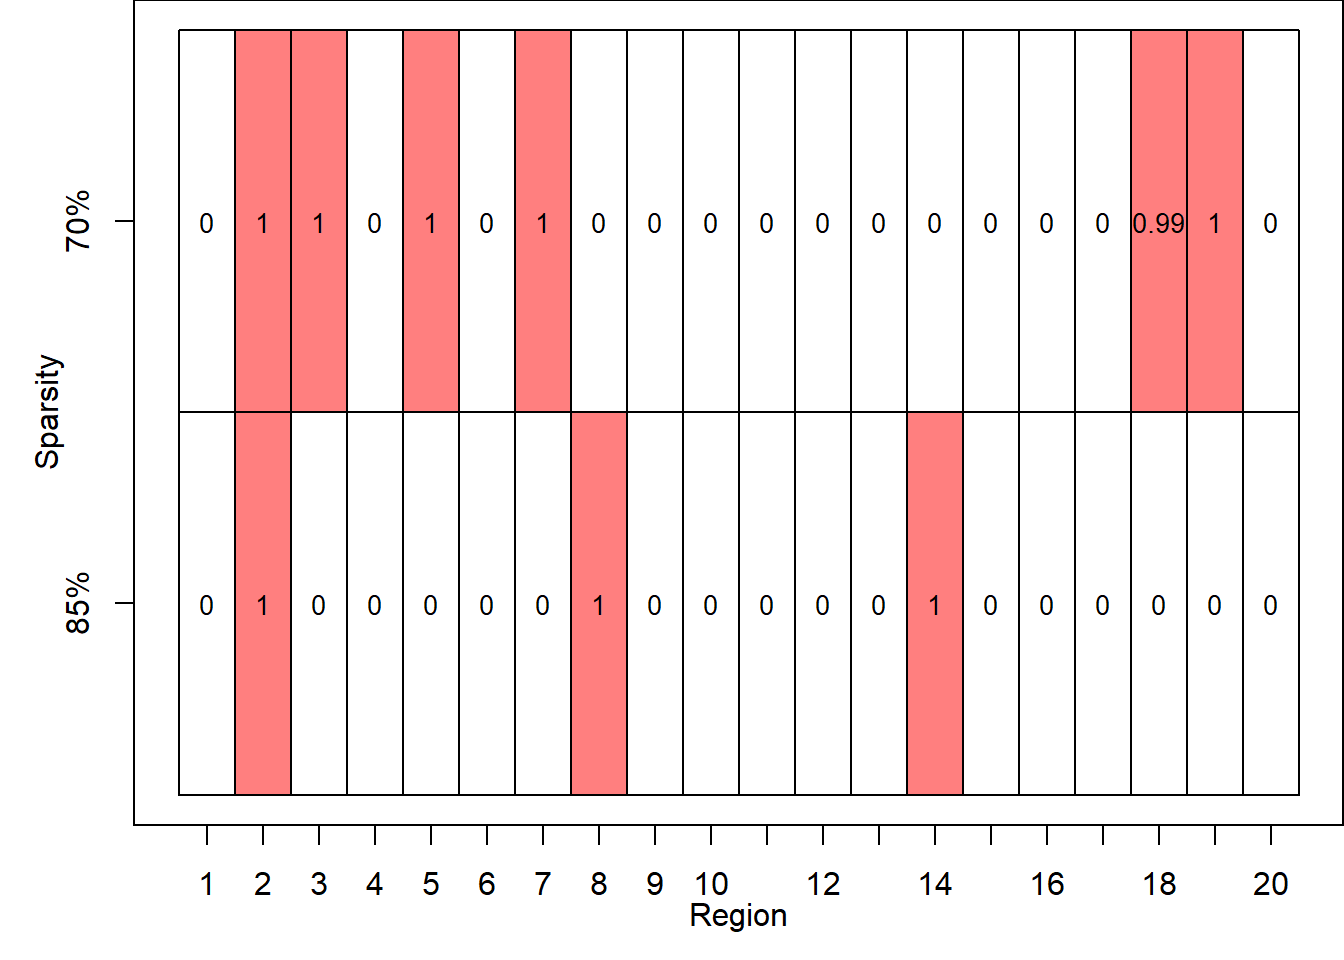
\includegraphics{_main_files/figure-latex/unnamed-chunk-3-1.pdf}

This file is available to edit as 04-example at \href{https://github.com/Rene-Gutierrez/bmrr}{Github}.

  \bibliography{references.bib}

\end{document}
